\chapter{Sequential Monte Carlo for Bayesian Computation}
\label{cha:Sequential Monte Carlo for Bayesian Computation}

As reviewed in chapter~\ref{cha:Monte Carlo Methods}, \mcmc algorithms, though
widely used for the purpose of Bayesian computation, have many limitations.
Algorithms such as \rjmcmc are conceptually appealing, yet often difficult to
design in practice. Other algorithms such as the Metropolis-Hastings algorithm
and Gibbs sampler, though provide generic frameworks which can be applied in
many fields, the design of efficient, high performance algorithms still
requires considerable expertise and sometimes extensive experience.

In recent years, there is a tendency of considering population based
algorithms. A common theme in these algorithms is that, instead of simulating
directly from complex target distribution, related yet simpler distributions
are used to ``help'' the simulation. One of such algorithm, which is
essentially a generalization of the Metropolis-Hastings algorithm, \pmcmc is
reviewed in section~\ref{sub:Population mcmc}, in which the easier to simulate
distribution ``lends'' information to the target and fastens its mixing.
Another example of population based algorithm is the recent development of
particular \mcmc \cite{Andrieu:2010gc}, which embed \smc samplers inside \mcmc
algorithms. The \smc sampler will be the central topic of this chapter

Sequential Monte Carlo (\smc) samplers, in various forms has been around for
more than a decade and widely used in many fields. Until recent there is
little interest of using it for Bayesian model comparison for a few reasons.
One of the more important one is that, when \mcmc algorithms are available,
\smc could cost more computational resources than a well designed \mcmc
algorithm. However we believe there are at least two important reasons that
\smc can be preferable to \mcmc for the purpose of Bayesian model comparison.
First, it provides a generic and robust framework for simulation from complex
distributions that are previously difficult for \mcmc algorithms, especially
for high dimensional multimodal distributions. Though it is not impossible to
design \mcmc algorithms for the same problems, it can be hugely difficult in
practice. The \smc framework provides a vital alternative that is easy to use.
It has the potential to enable statisticians to construct more realistic,
useful models that were previously difficult, if not impossible, to use due to
the computational complexity. Second, most Monte Carlo algorithms has to be
implemented on computers to be useful. Therefore it is unrealistic to not
consider the trend of today's computer technologies. Parallel computing has
become commodity in recent years. And \smc is much more suitable for this kind
of computing than conventional \mcmc. And as we will see later, \smc has
certain advantage over some other parallelized algorithms.

In this chapter, we first give a review of \smc algorithms in
section~\ref{sec:Sequential Monte Carlo samplers}. It is followed by a section
details the use of \smc in the context of Bayesian model comparison. Next,
section~\ref{sec:Extensions and refinements} develops some extensions and
refinements of existing practices. It is followed by a discussion of how the
presented framework lead to an automatic and generic algorithms. This chapter
is concluded with an extensive performance studies of various proposed
strategies.

\section{Sequential Monte Carlo samplers}
\label{sec:Sequential Monte Carlo samplers}

\smc samplers allow us to obtain, iteratively, collections of weighted samples
from a sequence of distribution $\{\pi_t\}_{t\ge0}$ over essentially any
random variables on some measurable spaces $(E_t,\calE_t)$. It is an extension
of the \emph{sequential importance sampling} (\sis) technique, which is a
generalization of particle filter algorithms widely used in physics and signal
tracking literature. In the remaining of this section, the sequential
importance sampling and resampling algorithms are introduced. Then how they
are generalized to \smc samplers for the purpose of the current work are
discussed.

\subsection{Sequential importance sampling and resampling}
\label{sub:Sequential importance sampling and resampling}

Sequential importance sampling (\sis) generalizes the importance sampling (see
section~\ref{sec:Classical Monte Carlo and importance sampling}) technique for
a sequence of distributions $\{\pi_t\}_{t\ge0}$ defined on spaces
$\{\prod_{k=0}^tE_k\}_{t\ge0}$. At time $t = 0$, sample
$\{X_0^{(i)}\}_{i=1}^N$ from $\eta_0$ and compute the weights $W_0^{(i)}
\propto \pi_0(X_0^{(i)})/\eta_0(X_0^{(i)})$. At time $t\ge1$, each sample
$X_{0:t-1}^{(i)}$, usually termed \emph{particles} in the literature, is
extended to $X_{0:t}^{(i)}$ by a proposal distribution
$q_t(\cdot|X_{0:t-1}^{(i)})$. And the weights are recalculated by $W_t^{(i)}
\propto \pi_t(X_{0:t}^{(i)})/\eta_t(X_{0:t}^{(i)})$ where
\begin{equation}
  \eta_t(X_{0:t}^{(i)}) =
  \eta_{t-1}(X_{0:t-1}^{(i)})q_t(X_{0:t}^{(i)}|X_{0:t-1}^{(i)})
\end{equation}
and thus
\begin{align}
  W_t^{(i)} \propto \frac{\pi_t(X_{0:t}^{(i)})}{\eta_t(X_{0:t}^{(i)})}
  &= \frac{\pi_t(X_{0:t}^{(i)})\pi_{t-1}(X_{0:t-1}^{(i)})}
  {\eta_{t-1}(X_{0:t-1}^{(i)})q_t(X_{0:t}^{(i)}|X_{0:t-1}^{(i)})
    \pi_{t-1}(X_{0:t-1}^{(i)})} \notag\\
  &= \frac{\pi_t(X_{0:t}^{(i)})}
  {q_t(X_{0:t}^{(i)}|X_{0:t-1}^{(i)})\pi_{t-1}(X_{0:t-1}^{(i)})}W_{t-1}^{(i)}
  \label{eq:si}
\end{align}
and importance sampling estimate of $\Exp_{\pi_t}[\varphi_t(X_{0:t})]$ can be
obtained using $\{W_t^{(i)},X_{0:t}^{(i)}\}_{i=1}^N$.

However this approach fails as $t$ becomes large. The weights tend to become
concentrated on a few particles as the discrepancy between $\eta_t$ and
$\pi_t$ becomes larger. Resampling techniques are applied such that, a new
particle system $\{\bar{W}_t^{(i)},\bar{X}_{0:t}^{(i)}\}_{i=1}^M$ is obtained
with the property,
\begin{equation}
  \Exp\Bigl[\sum_{i=1}^M\bar{W}_t^{(i)}\varphi_t(\bar{X}_{0:t}^{(i)})\Bigr] =
  \Exp\Bigl[\sum_{i=1}^NW_t^{(i)}\varphi_t(X_{0:t}^{(i)})\Bigr]
  \label{eq:resample}
\end{equation}
In practice, the resampling algorithm is usually chosen such that $M = N$ and
$\bar{W}^{(i)} = 1/N$ for $i=1,\dots,N$. Resampling can be performed at each time
$t$ or adaptively based on some criteria of the discrepancy. One popular
quantity used to monitor the discrepancy is \emph{effective sample size}
(\ess), introduced by \cite{Liu:1998iu}, defined as
\begin{equation}
  \ess_t = \frac{1}{\sum_{i=1}^N (W_t^{(i)})^2}
\end{equation}
where $\{W_t^{(i)}\}_{i=1}^N$ are the normalized weights. And resampling can
be performed when $\ess\le \alpha N$ where $\alpha\in[0,1]$.

The common practice of resampling is to replicate particles with large weights
and discard those with small weights. In other words, instead of generating a
random sample $\{\bar{X}_{0:t}^{(i)}\}_{i=1}^N$ directly, a random sample of
integers $\{R_t^{(i)}\}_{i=1}^N$ is generated, such that $R_t^{(i)} \ge 0$ for
$i = 1,\dots,N$ and $\sum_{i=1}^N R_t^{(i)} = N$. And each particle value
$X_{0:t}^{(i)}$ is replicated for $R_t^{(i)}$ times in the new particle
system.  The distribution of $\{R_t^{(i)}\}_{i=1}^N$ shall fulfill the
requirement of Equation~\ref{eq:resample}. One such distribution is a
multinomial distribution of size $N$ and weights
$(W_t^{(i)},\dots,W_t^{(N)})$. See \cite{Douc:2005wa} for some commonly used
resampling algorithms. Here we briefly review some of the most commonly used
algorithms besides the multinomial resampling.

\paragraph{Residual resampling} It was introduced in \cite{Liu:1998iu}. In
this approach, for $i = 1,\dots,N$, we have
\begin{equation}
  R_t^{(i)} = \Floor{NW_t^{(i)}} + \bar{R}_t^{(i)}
\end{equation}
where $\Floor{}$ denotes the integer part and $\{R_t^{(i)}\}_{i=1}^N$ are
distributed according to a multinomial distribution with size $N - \bar{N}_t$
and weights $(\bar{W}_t^{(i)},\dots,\bar{W}_t^{(N)})$ with
\begin{align*}
  \bar{N}_t &= \sum_{i=1}^N\Floor{NW_t^{(i)}} \\
  \bar{W}_t^{(i)} &= \frac{NW_t^{(i)} - \Floor{NW_t^{(i)}}}{N - \bar{N}_t}
\end{align*}
It was shown that residual resampling can lead to significant variance
reduction when compared to multinomial resampling. It is easy to see that,
unlike multinomial resampling, in residual resampling, the replication number
$R_t^{(i)}$ will differ from $NW_t^{(i)}$ by at most $1$. The next two
resampling algorithms also share this property.

\paragraph{Stratified resampling} Let $Q$ denote the inverse of the cumulative
distribution of a multinomial distribution with size $N$ and eights
$(W_1,\dots,W_N)$, the stratified resampling proceed by first drawing uniform
random variates $U_t^{(i)}$ on $((i-1)/N, i/N]$ for $i = 1,\dots,N$, and then
generate $I_t^{(i)} = Q(U_t^{(i)})$. The new particles system is formed by
$\{X_{0:t}^{(I_t^{(i)})}\}_{i=1}^N$.  This algorithm also outperforms the
multinomial resampling.

\paragraph{Systematic resampling} Similar to the stratified resampling, the
systematic resampling also use the inversion method. However, instead of
generating $N$ uniform random variates, it only generates one uniform random
variate $U_t$ from $(0, 1/N]$ and deterministically set $U_t^{(i)} = (i - 1)/N
+ U_t$. Though it has the most simplistic implementation among all algorithms
introduced so far, it is more complicated to study the behavior of the
conditional variance of the generated samples. As shown in \cite{Douc:2005wa},
there exists counter-examples that the systematic resampling does not
outperform the multinomial resampling.

\paragraph{Combination of residual and stratified/systematic resampling} Both
the stratified and systematic resampling algorithms can be used together with
the residual resampling. It operates by first compute the integer part and
residuals of $NW_t^{(i)}$, and then stratified or systematic resampling are
performed using the residuals as weights. It has the advantage that the
resulting algorithm provide better performance the then residual resampling or
the stratified or systematic resampling.

There are other specialized resampling algorithms. The algorithms shown above
has a common drawback. They requires the knowledge of all the weights being
available before the algorithm can proceed. Therefore in some situations the
performance of \smc algorithms can be limited by the fact that the resampling
step cannot be parallelized. Parallelized resampling algorithms is an area
that is actively researched. However, we will not discuss such specialized
algorithms in this work.

\subsection[SMC samplers]{\protect\smc samplers}
\label{sub:SMC Samplers}

\smc samplers generates the \sis algorithm for a sequence of distributions
$\{\pi_t\}_{t\ge0}$ over essentially any random variables on some spaces
$\{E_t\}_{t\ge0}$, by constructing a sequence of auxiliary distributions
$\{\tilde\pi_t\}_{t\ge0}$ on spaces of increasing dimensions,
\begin{equation}
  \tilde\pi_t(x_{0:t})=\pi_t (x_t) \prod_{s=0}^{t-1} L_s(x_{s+1},x_s),
\end{equation}
where the sequence of Markov kernels $\{L_s\}_{s=0}^{t-1}$, termed backward
kernels, is formally arbitrary but critically influences the estimator
variance. See \cite{DelMoral:2006hc} for further details and guidance on the
selection of these kernels (also see section~\ref{sub:Optimal and suboptimal
  backward kernels}.)

Standard sequential importance sampling and resampling algorithms can then be
applied to the sequence of synthetic distributions, $\{\tilde\pi_t\}_{t\ge0}$.
At time $t - 1$, assume that a set of weighted particles
$\{W_{t-1}^{(i)},X_{0:t-1}^{(i)}\}_{i=1}^N$ approximating $\tilde\pi_{t-1}$ is
available, then at time $t$, the path of each particle is extended with a
Markov kernel say, $K_t(x_{t-1}, x_t)$ and the set of particles
$\{X_{0:t}^{(i)}\}_{i=1}^N$ reach the distribution $\eta_t(X_{0:t}^{(i)}) =
\eta_0(X_0^{(i)})\prod_{k=1}^tK_t(X_{t-1}^{(i)}, X_t^{(i)})$, where $\eta_0$
is the initial distribution of the particles. To correct the discrepancy
between $\eta_t$ and $\tilde\pi_t$, equation~\ref{eq:si} is applied and in
this case,
\begin{equation}
  W_t^{(i)} \propto \frac{\tilde\pi_t(X_{0:t}^{(i)})}{\eta_t(X_{0:t}^{(i)})}
  = \frac{\pi_t(X_t^{(i)})\prod_{s=0}^{t-1}L_s(X_{s+1}^{(i)}, X_s^{(i)})}
  {\eta_0(X_0^{(i)})\prod_{k=1}^tK_k(X_{k-1}^{(i)},X_k^{(i)})}
  \propto \tilde{w}_t(X_{t-1}^{(i)}, X_t^{(i)})W_{t-1}^{(i)}
\end{equation}
where $\tilde{w}_t$, termed the \emph{incremental weights}, are calculated as,
\begin{equation}
  \tilde{w}_t(X_{t-1}^{(i)},X_t^{(i)}) =
  \frac{\pi_t(X_t^{(i)})L_{t-1}(X_t^{(i)}, X_{t-1}^{(i)})}
  {\pi_{t-1}(X_{t-1}^{(i)})K_t(X_{t-1}^{(i)}, X_t^{(i)})}
\end{equation}
If $\pi_t$ is only known up to a normalizing constant, say $\pi_t(x_t) =
\gamma_t(x_t)/Z_t$, then we can use the \emph{unnormalized} incremental
weights
\begin{equation}
  w_t(X_{t-1}^{(i)},X_t^{(i)}) =
  \frac{\gamma_t(X_t^{(i)})L_{t-1}(X_t^{(i)}, X_{t-1}^{(i)})}
  {\gamma_{t-1}(X_{t-1}^{(i)})K_t(X_{t-1}^{(i)}, X_t^{(i)})}
\end{equation}
for importance sampling. Further, with the previously \emph{normalized}
weights $\{W_{t-1}^{(i)}\}_{i=1}^N$, we can estimate the ratio of normalizing
constant $Z_t/Z_{t-1}$ by
\begin{equation}
  \frac{\hat{Z}_t}{Z_{t-1}} =
  \sum_{i=1}^N W_{t-1}^{(i)}w_t(X_{t-1}^{(i)},X_t^{(i)})
  \label{eq:ratio normalized}
\end{equation}
Sequentially, the normalizing constant between initial distribution $\pi_0$
and some target $\pi_T$, $T\ge1$ can be estimated. See \cite{DelMoral:2006hc}
and section~\ref{sub:Optimal and suboptimal backward kernels} for details on
calculating the incremental weights.

\subsection{Sequence of distributions}
\label{sub:Sequence of distributions}

There are many ways to specify the sequence of distributions. For many
applications, such a sequence arises from the problem setting naturally.

In \cite{Chopin:2002hg}, a data tempering scheme was considered in the context
of Bayesian inference for static parameters. Suppose data $\data =
(y_1,\dots,y_n)$ are available and the interest is to inference the posterior
distribution of some parameter vector $\theta$, $\pi(\theta|\data)$. Then one
can construct the following sequence of distributions $\{\pi_t\}_{t=1}^n$,
\begin{equation}
  \pi_t(\theta) = \pi(\theta|y_1,\dots,y_t).
\end{equation}
That is, the data is introduced one by one into the posterior. However, this
scheme can be sensitive to the order of data being introduced. A modification
is to introduce a batch of data at each iteration, also introduced in
\cite{Chopin:2002hg}. How many data points to be incorporated in each
iteration can still be difficult to determine. The more data points introduced
at each step, the more degeneracy (measured by, e.g., \ess) will be induced.
It is natural to consider introduce data such that a constant level of
degeneracy is maintained. It is intuitive to see that with enough data (large
$t$), the addition of the same amount of data will have less influence on the
posterior than when there are only a few data (small $t$) being introduced.
It was shown in \cite{Chopin:2002hg} that, under this assumption, it can be
expected that the number of data points at each step increase geometrically.

Another generic scheme is commonly called the \emph{geometric path}. Given the
target distribution $\pi$ and another distribution $\eta$, which usually has
the same support but heavier tail than $\pi$, a sequence of distributions
$\{\pi_t\}_{t=0}^T$ can be constructed,
\begin{equation}
  \pi_t(x) =
  \pi(x)^{\alpha(t/T)}\eta(x)^{1-\alpha(t/T)} \end{equation} where
$\alpha:[0,1]\to[0,1]$ is a monotonic increasing mapping with $\alpha(0) = 0$
and $\alpha(1) = 1$. Some variants of this scheme adapted particularly for the
purpose of Bayesian modeling can be seen in section~\ref{sub:smc1: An
  all-in-one approach} and~\ref{sub:smc2: A direct-evidence-calculation
  approach}. The sequence of distributions moves smoothly from $\eta$, which
is usually easy to sample from or to construct an efficient instrumental
distribution for, towards the target distribution $\pi$. However, this scheme
does has one important drawback. For high dimensional target with many well
separated modes, it can be difficult for $\eta$ (or its instrumental
distribution) to produce samples within each of all the modes and thus sampler
may never reach some of the space of the target $\pi$. This problem can be
partially solved by increase the number of particles.

Despite this limitation, the geometric scheme has a significant advantage as
we will see later (section~\ref{sub:Optimal and suboptimal backward kernels}
and~\ref{sub:Adaptive specification of distributions}). In short, when
combined with certain transition kernels and backward kernels, it allows easy
computation of the weights using quantities already computed in the last
iteration without actually simulate the samples. Therefore it provides a way
to conduct adaptive sampling at low computational cost.

There are other sequences, which often has particular use for certain
applications. For example, for global optimization of a function $f$, such
that $\int f(x)\intd x <\infty$ (that is, it can be normalized into a density
function), one can simulate from a sequence of distribution,
\begin{equation}
  \pi_t(x) \propto f(x)^{\alpha_t}
\end{equation}
where $\alpha_t$ is an increasing sequence and $\alpha_t\to\infty$ as
$t\to\infty$. The sequence of distributions will concentrate more and more
around the mode of $f$.

\subsection{Sequence of transition kernels}
\label{sub:Sequence of transition kernels}

It is easy to see that, the optimal proposal kernel is $K_t(x_{t-1}, x_t) =
\pi_t(x_t)$, in the sense of minimizing the Monte Carlo variance of the
importance weights. However, this choice is not possible except for trivial
toy examples. Some sensible alternatives have been proposed in the past.

One approach is to use independent proposals, $K_t(x_{t-1}) = \mu_t(x_{t-1})$
for some distribution $\mu_t$ at each iteration. Usually, $\mu_t$ belongs to a
family of distributions with parameters determined by certain statistics of
$\eta_{t-1}$. For example, a multivariate Normal distribution with mean vector
and covariance matrix estimated from current samples. This approach is most
commonly seen in the particle filter literature, where often the problems
provide natural candidate of the distribution $\mu_t$. However, for more
general use, this can be overly restrictive and the performance can be
difficult to calibrate, especially in high dimensional problems. In this
situation, it is difficult for the independent proposal to capture the
characteristics of target distribution without knowing it in advance. And thus
it can lead to large variance of importance weights and poor performance of
the sampler.

An important alternative, advocated in \cite{DelMoral:2006hc} is to use \mcmc
kernels targeting $\pi_t$. This strategy is particularly justified if the
sequence of distributions moves smoothly or the kernel is fast mixing. When the
sequence of distributions moves slowly from one to another, that is $\pi_t$
is not very different from $\pi_{t-1}$, and thus samples from $\eta_{t-1}$ is
a good approximation for $\pi_t$, the kernel is likely to successfully move
particles towards high probability regions of $\pi_t$. What makes it more
attractive is the fact that we can use the vast literature on the design of
efficient \mcmc algorithms to build the importance distribution. In addition,
as we will see very soon, when combined with certain backward kernels, this
approach enables us to calculate the importance weights without actually
simulate samples. And therefore it leads to low computational cost adaptive
algorithms that can improve the performance considerably.

\subsection{Optimal and suboptimal backward kernels}
\label{sub:Optimal and suboptimal backward kernels}

The backward kernel $\{L_t\}_{t=0}^{T-1}$ should be optimized with respect to
the transition kernel $\{K_t\}_{t=0}^T$. As shown in proposition~1{} in
\cite{DelMoral:2006hc}, the backward kernel $L_{t-1}(x_t, x_{t-1})$ that
minimize the variance of unnormalized importance weights is given by,
\begin{equation}
  \Lopt{t-1}(x_t,x_{t-1}) =
  \frac{\eta_{t-1}(x_{t-1})K_t(x_{t-1},x_t)}{\eta_t(x_t)}
\end{equation}
and in this case the weights,
\begin{equation}
  W_t(X_{t-1},X_t) \propto \pi_t(x_t)/\eta_t(x_t)
\end{equation}
where $\eta_t(x_t)$ is the marginal of $\eta_t(x_{0:t})$. This marginal is
typically not available and thus the above optimal backward kernel cannot be
used in practice.

One sensible alternative is to substitute $\pi_{t-1}$ for $\eta_{t-1}$, that
is,
\begin{equation}
  L_{t-1}(x_t,x_{t-1}) =
  \frac{\pi_{t-1}(x_{t-1})K_t(x_{t-1},x_t)}
  {\int \pi_{t-1}(x_{t-1})K_t(x_{t-1},x_t)\intd x_{t-1}}
  \label{eq:subopt back kernel}
\end{equation}
This approach is justified if the particles has been resampled at time $t-1$,
in which case $\eta_{n-1}$ is indeed approximately equal to $\pi_{n-1}$ or
when resampling was at least performed occasionally such that the degeneracy
between $\eta_{t-1}$ and $\pi_{t-1}$ is controlled. The incremental weights
can be computed if the integration above can be computed.  Usually this is
done through the unnormalized distribution $\gamma_{t-1}$ instead of
$\pi_{t-1}$. When $\gamma_{t-1}$ is known analytically, the unnormalized
incremental weights are,
\begin{equation}
  w_t(X_{t-1}^{(i)},X_t^{(i)}) =
  \frac{\gamma_t(X_t^{(i)})}
  {\int\gamma_{t-1}(x_{t-1})K_t(x_{t-1},X_t^{(i)})\intd x_{t-1}}.
  \label{eq:inc weight subopt}
\end{equation}
The requirement of the knowledge of the above integration can limit the use of
the kernel in many applications.

When using \mcmc kernels $K_t$ that is invariant to $\pi_t$ as transitional
kernels, and when $\pi_{t-1}\approx\pi_t$, by substitute $\pi_t$ for
$\pi_{t-1}$, equation~\eqref{eq:subopt back kernel} becomes,
\begin{align}
  L_{t-1}(x_t,x_{t-1})
  &= \frac{\pi_t(x_{t-1})K_t(x_{t-1},x_t)}
  {\int \pi_t(x_{t-1})K_t(x_{t-1},x_t)\intd x_{t-1}} \notag\\
  &= \frac{\pi_t(x_{t-1}K_t(x_{t-1},x_t)}{\pi_t(x_t)}
  \label{eq:subopt back kernel mcmc}
\end{align}
where the second equation is due to the fact that $K_t$ is invariant to
$\pi_t$. It is easy to see that the unnormalized incremental weights are,
\begin{equation}
  w_t(X_{t-1}^{(i)},X_t^{(i)}) =
  \frac{\gamma_t(X_{t-1}^{(i)})}{\gamma_{t-1}(X_{t-1}^{(i)})}.
  \label{eq:inc weight subopt mcmc}
\end{equation}
Note that, the incremental weights no longer depend on the samples from
iteration $t$, $\{X_t^{(i)}\}$. Therefore, it can be calculated before the
sampling step, which moves the particles according to the kernel $K_t$. Since
the incremental weights solely depends on the specification of $\gamma_t$,
which usually can be computed point-wise, given the current samples, it is
possible to specify $\gamma_t$ (and $\pi_t$) according to the calculated
weights using informations from the current samples before carrying out the
actual simulations of the current iteration.

However the expression~\eqref{eq:inc weight subopt mcmc} is not without
drawbacks. Compared to the expression~\eqref{eq:inc weight subopt}, which is
more intuitive since it considers the transition kernel $K_t$ which depends on
the current samples, it benefits less from fast mixing kernels. If $\pi_t$ is
not close to $\pi_{t-1}$, then the variance of the incremental weights is
likely to be large even the kernel $K_t$ mixes fast. Indeed, later we will
show empirically that, it is preferable to use more distributions rather than
using multiple passes of \mcmc moves in a single iteration, provided that they
use the same computational resources.

\section{Application to Bayesian model comparison}
\label{sec:Application to Bayesian model comparison}

The application of \smc samplers to the Bayesian model comparison problem is
straightforward. However, it has been overlooked in recent years. In this
section, we outline common strategies of using \smc samplers for Bayesian
model comparison. In the next section, we introduce some innovative refinement
and extensions to existing practices.

The problem of interest is characterizing the posterior distribution over
$\{\Mk\}_{k\in\calK}$, a set of possible models, with model $\Mk$ having
parameter vector $\paramk\in\Paramk$ which must also usually be inferred.
Given prior distributions $\pi(\Mk)$ and $\pi(\paramk|\Mk)$ and likelihood
$p(\data|\paramk,\Mk)$ we seek the posterior distributions $\pi(\Mk|\data)
\propto p(\data|\Mk)\pi(\Mk)$. There are three fundamentally different
approaches to the computations,
\begin{enumerate}
  \item Calculate posterior model probabilities directly.
  \item Calculate the evidence, $p(\data|\Mk)$, of each model.
  \item Calculate pairwise evidence ratios.
\end{enumerate}
Each approach admits a natural \smc strategy.

\subsection{\smc[1]: An all-in-one approach}
\label{sub:smc1: An all-in-one approach}

One could consider obtaining samples from the same distribution employed in
the \rjmcmc approach to model comparison, namely,
\begin{equation}
  \pi^{(1)}(\Mk,\paramk) \propto \pi(\Mk)\pi(\paramk|\Mk)p(\data|\paramk,\Mk)
\end{equation}
which is defined on the disjoint union space
$\bigcup_{k\in\calK}(\{\Mk\}\times\Paramk)$.

One obvious \smc approach is to define a sequence of distributions
$\{\pi_t^{(1)}\}_{t=0}^T$ such that $\pi^{(1)}_0$ is easy to sample from,
$\pi_{T}^{(1)} = \pi^{(1)}$ and the intermediate distributions move smoothly
between them. In the remainder of this section, we use the notation
$(\Mk[t],\paramk[t])$ to denote a random sample on the space
$\bigcup_{k\in\calK}(\{\Mk\}\times\Paramk)$ at time $t$. One simple approach,
which might be expected to work well, is the use of an annealing scheme such
that,
\begin{equation}
  \pi^{(1)}_t(\Mk[t],\paramk[t]) \propto \pi(\Mk[t])\pi(\paramk[t]|\Mk[t])
  p(\data|\paramk[t],\Mk[t])^{\alpha(t/T)},
  \label{eq:geometry_1}
\end{equation}
for some monotonically increasing $\alpha:[0,1]\to[0,1]$ such that $\alpha(0)
= 0$ and $\alpha(1) = 1$. Other approaches are possible and might prove more
efficient for some problems (such as the ``data tempering'' approach which
\cite{Chopin:2002hg} proposed for parameter estimation which could easily
be incorporated in our framework), but this strategy provides a convenient
generic approach. These choices lead to Algorithm~\ref{alg:smc1}.

% $\alpha$ provides an \emph{annealing schedule} which is intended to allow
% the control of the discrepancy between pairs of adjacent distributions. This
% gives the joint prior on model order and parameters as an initial
% distribution and gradually introduces the influence of the likelihood until
% the full posterior is reached.

% Given a weighted collection of samples $\{W^{(k,i)}_T, X^{(k,i)}_{T} =
% (K_T^{(k,i)},\theta_T^{(k,i)})\}_{i=1}^N$ targeting $\pi^{(1)}$, one may
% approximate the two distributions of interest using the empirical measures,
% \begin{align*}
%   \hat{\pi}^{(1)}(K = k) &= \sum\limits_{i=1}^N W^{(k,i)} \delta_{k,
%   K^{(k,i)}_T} \\
%   \hat{\pi}^{(1)}(d\theta|K=k) &= \frac{1}{\hat{\pi}^{(1)}(K = k)}
%   \sum\limits_{i=1}^N W^{(k,i)} \delta_{k, K_T^{(k,i)}}
%   \delta_{\theta^{(k,i)}_T}(d\theta),
% \end{align*}
% where $\delta_{k,K^{(k,i)}_T}$ denotes the \emph{Kronecker} delta and
% $\delta_{\theta{(k,i)}}$ denotes the Dirac measure concentrated at
% $\theta^{(k,i)}$.

% Thus, the output of such an \smc algorithm may be used as a (weighted)
% equivalent to that from a suitable \rjmcmc algorithm, with the posterior
% probability of each model corresponding to the (weighted) proportion of
% samples from that model.

This approach might outperform \rjmcmc when it is difficult to design
fast-mixing Markov kernels. There are many examples of such an annealed \smc
strategy outperforming \mcmc at a given computational cost -- see, for
example, \cite{Fan:2008tf,Johansen:2008kp,Fearnhead:2010ua}. Such
trans-dimensional \smc has been proposed in several contexts
\cite{Peters:2005wh} and an extension proposed and analysed
by \cite{Jasra:2008bb}.

\begin{algorithm}
\begin{algorithmic}
  \tophrule
  \STATE \emph{Initialisation:} Set $t\leftarrow0$.
  \STATE\STATESKIP Sample $X_0^{(i)} = (M_0^{(i)},\theta_0^{(i)})\sim\nu$
  for some proposal distribution $\nu$ (usually the joint prior).
  \STATE\STATESKIP Weight $W_0^{(i)} \propto w_0(X_0^{(i)}) =
  {\pi(M_0^{(i)}) \pi(\theta^{(i)}_0|M_0^{(i)})}/
  {\nu(M_0^{(i)},\theta_0^{(i)})}$.
  \STATE\STATESKIP Apply resampling if necessary (e.g., if \ess
  \cite{Kong:1994ul} less than some threshold).

  \STATE \emph{Iteration:} Set $t\leftarrow t + 1$.
  \STATE\STATESKIP Weight $W_t^{(i)} \propto W_{t-1}^{(i)}
  p(\data|\theta_{t-1}^{(i)},M_{t-1}^{(i)})^{\alpha(t/T) - \alpha([t-1]/T)}$.
  \STATE\STATESKIP Apply resampling if necessary.
  \STATE\STATESKIP Sample $X_t^{(i)} \sim K_t(\cdot|X_{t-1}^{(i)})$, a
  $\pi_t^{(1)}$-invariant kernel.

  \STATE \emph{Repeat} the \emph{Iteration} step \emph{until $t = T$}.
  \bottomhrule
\end{algorithmic}
\caption{\smc[1]: An All-in-One Approach to Model Comparison.}
\label{alg:smc1}
\end{algorithm}

We include this approach for completeness and study it empirically later.
However, the more direct approaches described in the following sections lead
more naturally to easy-to-implement strategies with good performance.

\subsection{\smc[2]: A direct-evidence-calculation approach}
\label{sub:smc2: A direct-evidence-calculation approach}

An alternative approach would be to estimate explicitly the evidence
associated with each model. We propose to do this by sampling from a sequence
of distributions for each model: starting from the parameter prior and
sweeping through a sequence of distributions to the posterior.

Numerous strategies are possible to construct such a sequence of
distributions, but one option is to use for each model $\Mk$, $k\in\calK$, the
sequence $\{\pi_t^{(2,k)}\}_{t=0}^{T_k}$, defined by
\begin{equation}
  \pi_t^{(2,k)}(\paramk[t]) \propto
  \pi(\paramk[t]|\Mk)p(\data|\paramk[t],\Mk)^{\alpha_k(t/T_k)}.
  \label{eq:geometry_2}
\end{equation}
where the number of distribution $T_k$, and the annealing schedule,
$\alpha_k:[0,1]\to[0,1]$ may be different for each model. This leads to
Algorithm~\ref{alg:smc2}.

The estimator of the posterior model probabilities depends upon the approach
taken to estimate the normalizing constant. Direct estimation of the evidence
can be performed using the output of this \smc algorithm and the standard
unbiased estimator, termed \smc[2]-\ds below (see also
equation~\eqref{eq:ratio normalized}),
\begin{equation}\label{eq:smc2-ds}
  \sum_{i=1}^N \frac{\pi(\theta_0^{(k,i)}|\Mk)}{\nu(\theta_0^{(k,i)})} \times
  \prod_{t=2}^T \sum_{i=1}^N W_{t-1}^{(k,i)}
  p(\data|\theta_{t-1}^{(k,i)}\Mk)^{\alpha_k(t/T_k) - \alpha_k([t-1]/T_k)}
\end{equation}
where $W_{t-1}^{(k,i)}$ is the importance weight of sample $i$,
$\theta_{t-1}^{(k,i)}$, during iteration $t-1$ for model $\Mk$. An alternative
approach to computing the evidence is also worthy of consideration. As has
been suggested, and shown to perform well empirically previously \cite[see,
for example]{Johansen:2006wm}, it is possible to use all of the samples from
every generation of an \smc sampler to approximate the path sampling estimator
and hence to obtain an estimate of the ratio of normalizing constants.
Section~\ref{sub:Path Sampling via smc2/smc3} provides details.

The posterior distribution of the parameters conditional upon a particular
model can also be approximated with,
\begin{equation*}
  \hat{\pi}_{T_k}^{(2,k)}(\diff\theta) =
  \sum\limits_{i=1}^{N} W_{T_k}^{(k,i)}
  \delta_{\theta^{(k,i)}_{T_k}}(\diff\theta).
\end{equation*}
where $\delta_{\theta^{(k,i)}_{T_k}}$ is the Dirac measure.

% It is straightforward to use different numbers of samples, $N$, for each
% model when appropriate. in settings in which some models can be
% characterised substantially more easily than others.

This approach is appealing for several reasons. One is that it is designed to
estimate directly the quantity of interest: the evidence, producing a sample
from that distribution at the same time. Another advantage of this approach
over \smc[1] and the \rjmcmc approach is that it provides as good a
characterisation of each model as is required: it is possible to obtain a good
estimate of the parameters of every model, even those for which the posterior
probability is small. Perhaps most significant is the fact that this approach
does not require the design of proposal distributions or Markov kernels which
move from one model to another: each model is dealt with in isolation. Whilst
this may not be desirable in every situation, there are circumstances in which
efficient moves between models are almost impossible to devise.

This approach also has some disadvantages. In particular, it is necessary to
run a separate simulation for each model -- rendering it impossible to deal
with countable collections of models (although this is not such a substantial
problem in many interesting cases). The ease of implementation may often
offset this limitation.

\begin{algorithm}
\begin{algorithmic}
  \tophrule
  \STATE For each model $k \in \calK$ perform the following algorithm.

  \STATE \emph{Initialisation:} Set $t\leftarrow0$.
  \STATE\STATESKIP Sample $\theta_0^{(k,i)}\sim\nu_k$ for some proposal
  distribution $\nu_k$ (usually the parameter prior).
  \STATE\STATESKIP Weight $W_0^{(k,i)} \propto w_0(\theta_0^{(k,i)}) =
  {\pi(\theta_0^{(k,i)}|\Mk)}/{\nu_k(\theta_0^{(k,i)})}$.
  \STATE\STATESKIP Apply resampling if necessary.

  \STATE \emph{Iteration:} Set $t\leftarrow t + 1$.
  \STATE\STATESKIP Weight $W_t^{(k,i)} \propto W_{t-1}^{(k,i)}
  p(\data|\theta_{t-1}^{(k,i)},\Mk)^{\alpha(t/T_k) - \alpha([t-1]/T_k)}$.
  \STATE\STATESKIP Apply resampling if necessary.
  \STATE\STATESKIP Sample $\theta_t^{(k,i)} \sim
  K_t(\cdot|\theta_{t-1}^{(k,i)})$, a $\pi_t^{(k,2)}$-invariant kernel.

  \STATE \emph{Repeat} the \emph{Iteration} step \emph{until $t = T_k$}.
  \bottomhrule
\end{algorithmic}
\caption{\smc[2]: A Direct-Evidence-Calculation Approach.}\label{alg:smc2}
\end{algorithm}

\subsection{\smc[3]: A relative-evidence-calculation approach}
\label{sub:smc3: A relative-evidence-calculation approach}

A final approach can be thought of as \emph{sequential model comparison}.
Rather than estimating the evidence associated with any particular model, we
could estimate pairwise evidence ratios directly. The \smc sampler starts with
a initial distribution being the posterior of one model (which could comes
from a separate \smc sampler starting from its prior) and moves towards the
posterior of another related model. Then the sampler can continue towards
another related model.

Given a finite collection of models $\{\Mk\}$, $k\in\calK$, suppose the models
are ordered in a sensible way (e.g., $\Mk[k-1]$ is nested within $\Mk$ or
$\paramk$ is of higher dimension than $\paramk[k-1]$). For each
$k\in\calK$, we consider a sequence of distributions
$\{\pi_t^{(3,k)}\}_{t=0}^{T_k}$, such that $\pi_0^{(3,k)}(\Mk[],\paramk[]) =
\pi(\paramk[]|\data,\Mk) \mathbb{I}_{\{\Mk\}}(\Mk[])$ and $\pi_{T_k}^{(3,k)}(\Mk[],\paramk[]) =
\pi(\paramk[]|\data,\Mk[k+1]) \mathbb{I}_{\{\Mk[k+1]\}}(\Mk[]) = \pi_{0}^{(3,k+1)}(\Mk[],\paramk[])$.
When it is possible to construct a \smc sampler that iterates over this
sequence of distributions, the estimate of the ratio of normalizing constants
is the Bayes factor estimate of model $\Mk[k+1]$ in favour of model $\Mk$.

This approach is conceptually appealing, but requires the construction of a
smooth path between the posterior distributions of interest. The geometric
annealing strategy which has been advocated as a good generic strategy in the
previous sections is only appropriate when the support of successive
distributions is non-increasing. This is unlikely to be the case in
interesting model comparison problems.

In this paper we consider a sequence of distributions on the disjoint union
$\{\Mk,\Paramk\}\cup\{\Mk[k+1],\Paramk[k+1]\},$ with the sequence of
distributions $\{\pi_t^{(3,k)}\}_{t=0}^{T_k}$ defined as the full posterior,
\begin{equation}
  \pi_t^{(3,k)}(\Mk[t],\paramk[t]) \propto
  \pi_t(\Mk[t]) \pi(\paramk[t]|\Mk[t]) p(\data|\paramk[t],\Mk[t])
\end{equation}
where $\Mk[t]\in\{\Mk,\Mk[k+1]\}$ and the prior of models at time $t$,
$\pi_t(\Mk[t])$ is defined by
\begin{equation}
  \pi_t(\Mk[k+1]) = \alpha(t/T_k)
  \label{eq:smc3_prior}
\end{equation}
for some monotonically increasing $\alpha:[0,1]\to[0,1]$ such that $\alpha(0)
= 0$ and $\alpha(1) = 1$. It is clear that the \mcmc moves between iterations
need to be similar to those in the \rjmcmc or \smc[1] algorithms. The
difference is that instead of efficient exploration of the whole model space,
only moves between two models are required and the sequence of distributions
employed helps to ensure exploration of both model spaces. The algorithm for
this particular sequence of distribution is outlined in
Algorithm~\ref{alg:smc3}. It can be extended to other possible sequence of
distributions between models.

An advantage of this approach is that it provides direct estimate of the Bayes
factor which is of interest for model comparison purpose while not requiring
exploration of as complicated a space as that employed within \rjmcmc or
\smc[1]. The estimating of normalizing constant in \smc[3] can follows in
exactly the same manner as in the \smc[2] case. In \smc[3], the same
estimator provides a direct estimate of the Bayes factor.

%Note that the standard \smc unbiased estimator is in fact the
%ratio of normalizing constants between the initial distribution and the final
%distribution. In \smc[2], we initialised the system with the prior
%distribution and thus the estimates are directly the evidence for each model.


\begin{algorithm}
\begin{algorithmic}
  \tophrule
  \STATE \emph{Initialisation:} Set $k\leftarrow1$.
  \STATE\STATESKIP Use Algorithm~\ref{alg:smc2} to obtain weighted samples
  for $\pi_{T_1}^{(3,1)}$, the parameter posterior for model $\Mk[1]$

  \STATE \emph{Relative Evidence Calculation}
  \STATE\STATESKIP Set $k\leftarrow k + 1$, $t\leftarrow0$.
  \STATE\STATESKIP Denote current weighted samples as
  $\{W_0^{(k,i)},X_0^{(k,i)}\}_{i=1}^N$ where $X_0^{(k,i)} =
  (M_0^{(k,i)},\theta_0^{(k,i)})$
  \STATE\STATESKIP Apply resampling if necessary.

  \STATE\STATESKIP \emph{Iteration:} Set $t\leftarrow t + 1$.
  \STATE\STATESKIP\STATESKIP Weight $W_t^{(k,i)} \propto W_{t-1}^{(k,i)}
  {\pi_t(M_{t-1}^{(k,i)})}/{\pi_{t-1}(M_{t-1}^{(k,i)})}$.
  \STATE\STATESKIP\STATESKIP Apply resampling if necessary.
  \STATE\STATESKIP\STATESKIP Sample $(M_t^{(k,i)},\theta_t^{(ki)}) \sim
  K_t(\cdot|M_{t-1}^{(k,i)}\theta_{t-1}^{(k,i)})$, a $\pi_t^{(3,k)}$-invariant
  kernel.

  \STATE\STATESKIP \emph{Repeat the \emph{Iteration} step up to $t = T_k$}.

  \STATE \emph{Repeat} the \emph{Relative Evidence Calculation} step \emph{until
    sequentially all relative evidences are calculated}.
  \bottomhrule
\end{algorithmic}
\caption{\smc[3]: A Relative-Evidence-Calculation Approach to Model Comparison.}
\label{alg:smc3}
\end{algorithm}

\subsection{Path Sampling via \smc[2]/\smc[3]}
\label{sub:Path Sampling via smc2/smc3}

The estimation of the normalizing constant associated with our sequences of
distributions can be achieved by a Monte Carlo approximation to the \emph{path
  sampling} formulation given by \cite{Gelman:1998ei}. This is similar to the
technique for \pmcmc as described in section~\ref{sec:Bayesian computation
  with Markov chain Monte Carlo}. In the context of \smc, this approach is
also very closely related to the use of \ais for the same purpose
\cite{Neal:2001we} but as will be demonstrated below the incorporation of some
other elements of the more general \smc algorithm family can improve
performance at negligible cost. Recall that, given a parameter $\alpha$ which
defines a family of distributions, $\{p_{\alpha} = q_{\alpha} /
Z_\alpha\}_{\alpha \in [0,1]}$ which move smoothly from $p_0 = q_0 / Z_0$ to
$p_1 = q_1 / Z_1$ as $\alpha$ increases from zero to one, one can estimate the
logarithm of the ratio of their normalizing constants via a simple integral
relationship which holds under very mild regularity conditions,
\begin{equation}
  \log\biggl( \frac{Z_1}{Z_0} \biggr) =
  \int_{0}^{1} \Exp_\alpha \biggl[ \rnd{\log q_{\alpha}(\cdot)}{\alpha}
  \biggr] \intd\alpha, \label{eq:path_identity}
\end{equation}
where $\Exp_\alpha$ denotes expectation under $p_\alpha$. Note that the
sequence of distributions in the \smc[2] and \smc[3] algorithms above, can both be
interpreted as belonging to such a family of distributions, with $\alpha_t =
\alpha(t/T_k)$, where the mapping $\alpha:[0,1]\to[0,1]$ is again monotonic
with $\alpha(0) = 0$ and $\alpha(1) = 1$.

The \smc sampler provides us with a set of weighted samples obtained from a
sequence of distributions suitable for approximating this integral. At each
$t$ we can obtain an estimate of the expectation within the integral for
$\alpha(t/T)$ via the usual importance sampling estimator, and this integral
can then be approximated via numerical integration. Whenever the sequence
of distributions employed by \smc[3] has appropriate differentiability it is
also possible to employ path sampling to estimate, directly, the evidence
ratio via this approach applied to the samples generated by that algorithm. In
general, given an increasing sequence $\{\alpha_t\}_{t=0}^T$ where $\alpha_0 =
0$ and $\alpha_T = 1$, a family of distributions
$\{p_{\alpha}\}_{\alpha\in[0,1]}$ as before, and a \smc sampler that iterates
over the sequence of distribution $\{\pi_t = p_{\alpha_t} =
q_{\alpha_t}/Z_{\alpha_t}\}_{t=0}^T$, then with the weighted samples
$\{W_t^{(j)},X_t^{(j)}\}_{j=1}^N$, and $t = 0,\dots,T$, a path sampling
estimator of the ratio of normalizing constants $\Xi_T = \log(Z_1/Z_0)$
can be approximated (using an elementary trapezoidal scheme) by
\begin{equation}
  \hat\Xi_{T}^{N} = \sum_{t=1}^T
  \frac{1}{2}(\alpha_t - \alpha_{t - 1})(U_t^N + U_{t-1}^N)
  \label{eq:path_est}
\end{equation}
where
\begin{equation}
  U_t^N = \sum_{j=1}^N
  W_t^{(j)} \rnd{\log q_{\alpha}(X_t^{(j)})}{\alpha}\Bigm|_{\alpha = \alpha_t}
\end{equation}

We term these estimators \smc[2]-\ps and \smc[3]-\ps in the followings. The
combination of \smc and path sampling is somewhat natural and has been
proposed before, e.g., \cite{Johansen:2006wm} although not there in a Bayesian
context. Despite the good performance observed in the setting of rare
event simulation, the estimation of normalizing constants by this approach
seems to have received little attention in the literature. We suspect that
this is because of widespread acceptance of the suggestion of
\cite{DelMoral:2006hc}, that \smc doesn't outperform \ais when normalizing
constants are the object of inference or that of \cite{Calderhead:2009bd}
that all simulation-based estimators based around path sampling can be
expected to behave similarly. We will demonstrate below that these
observations, whilst true in certain contexts, do not hold in full generality.

\section{Extensions and refinements}
\label{sec:Extensions and refinements}

The algorithms introduced in the last section can be seen as straightforward
application of the well established \smc algorithms to Bayesian model
comparison. Though by construction, \smc algorithms can be more robust than
many \mcmc and other algorithms. However, as with any Monte Carlo algorithms,
without careful design, the performance can be far from satisfactory for many
realistic applications. In this section, we introduce some extensions and
refinement that can further improve the presented framework. Of course, they
cannot guarantee that the algorithms will perform well for all possible
situations. However, it provide robust and reliable solutions for many
realistic applications with minimal manual tuning. For more difficult
problems, they also provide a solid foundations on top of which higher
performance algorithms can be built.

We will use the \pet compartmental model example for illustrative purpose in
this section. More comprehensive performance comparisons can be found in
section~\ref{sub:Positron Emission Tomography compartmental model}. We will
consider both simulated and real world data. The simulated data set is the
same as in chapter~\ref{cha:Introduction}. Due to the large amount of the real
data, it is beyond the resources we have to perform repeated simulations for a
whole \pet scan. Instead, 20 real data sets are sampled from typical region of
interest in a single \pet scan. Figure~\ref{fig:typical real pet} shows three
of them. As we can see, they varies considerably in characteristics despite
all can be described as ``typical'' \pet data. The purpose of the current work
is to advocate robust and self-tuning algorithms. And the variability in the
data sets provides excellent test examples. In addition, in this chapter, the
models are configured with the non-informative priors and thus the parameters
are exchangeable, similar to that of a mixture model. This creates a
multimodal posterior surface for models with two or more components.

\begin{figure}[t]
  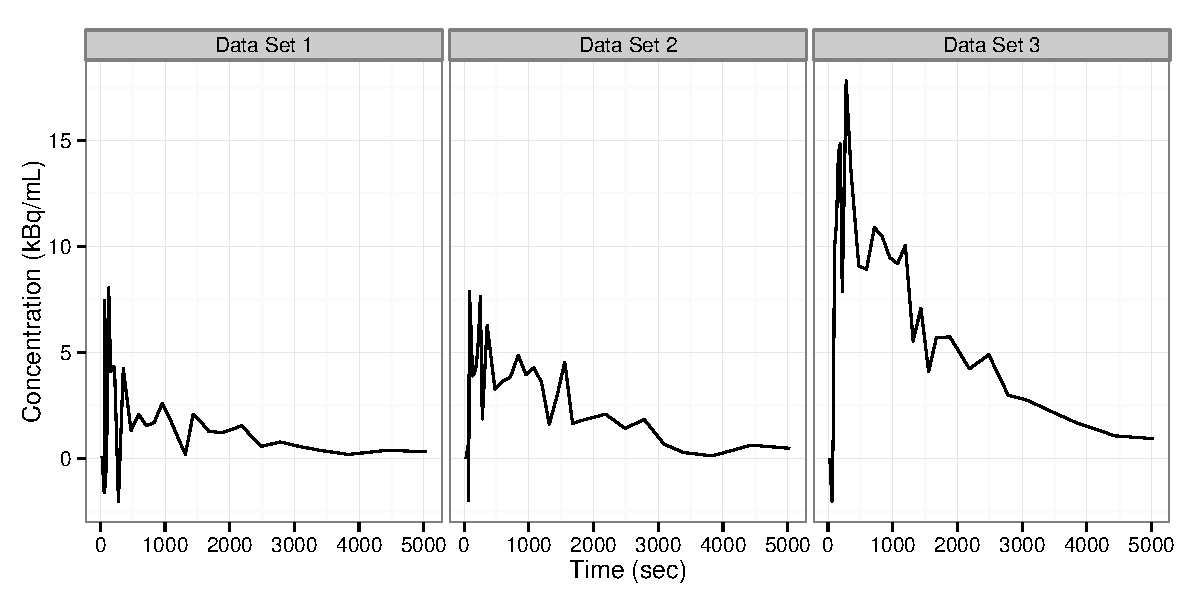
\includegraphics[width=\linewidth]{fig/Typical_PET}
  \caption{Typical real \pet data}
  \label{fig:typical real pet}
\end{figure}

\subsection{Improved univariate numerical integration}
\label{sub:Improved univariate numerical integration}

As seen in the last section, the path sampling estimator requires evaluation
of the expectation,
\begin{equation*}
  \Exp_\alpha \biggl[ \rnd{\log q_{\alpha}(\cdot)}{\alpha} \biggr]
\end{equation*}
for $\alpha\in[0,1]$, which can be approximated by importance sampling using
samples generated by a \smc sampler operating on the sequence of distributions
$\{\pi_t = p_{\alpha_t} = q_{\alpha_t}/Z_t\}_{t=0}^T$ directly for
$\alpha\in\{\alpha_t\}_{t=0}^T$. For arbitrary $\alpha\in[0,1]$, finding $t$
such that $\alpha\in(\alpha_{t-1},\alpha_t)$, the expectation can be easily
approximated using existing \smc samples -- the quantities required in the
importance weights to obtain such an estimate have already been calculated
during the running of the \smc algorithm and such computations have little
computational cost. %Indeed, in settings in which the \smc importance weights
%for target distribution $\pi_{\alpha}$ depend only upon the sample at time
%$t-1$, as in the proposed algorithms, the computational cost of the new
%weights are often minimal compared to generate new samples.

As noted by \cite{Friel:2012}  we can use more sophisticated numerical
integration strategies to reduce the path sampling estimator bias. For
example, higher order Newton-Cotes rules rather than the Trapezoidal rule can
be implemented straightforwardly. In the case of SMC it is especially
straightforward to estimate the required expectations at arbitrary $\alpha$
and so we cheaply use higher order integration schemes and we can also use
numerical integrations which make use of a finer mesh
$\{\alpha_t'\}_{t=0}^{T'}$ than $\{\alpha_t\}_{t=0}^T$. Since higher order
numerical integrations based on approximations of derivatives obtained from
Monte Carlo methods may potentially be unstable in some situations, the second
approach can be more appealing in some applications. A demonstration of the
bias reduction effect is provided in section~\ref{sub:Positron Emission
  Tomography compartmental model}.

% It is straightforwardly possible to use more sophisticated numerical
% integration techniques in order to evaluate the approximation of the path
% sampling estimator. Even in the presence of adaptive annealing schemes, it
% is reasonably straightforward to implement higher order schemes than the
% simple Trapezoidal approximation. In a related setting, this was shown to
% provide an appreciable reduction in bias by \cite{Friel:2012}. In our
% context we have found that the bias of even the simple Trapezoidal scheme is
% inconsequential in the regime in which the variance of this method is small
% enough to be competitive and so in the interests of parsimony we have not
% investigated such schemes.

% It is possible to use numerical integration methods other than the
% Trapezoidal rules to improve the path sampling estimator. For example, in a
% \smc[2] algorithm, if a sequence of distribution indexed by
% $\{\alpha(t/T)\}_{t=0}^T$ are used, where the path sampling integration is
% with respect to $\alpha\in[0,1]$. Then by placing an additional set of
% distributions at middle points
% $\{(\alpha(t/T)+\alpha((t+1)/T))/2\}_{t=0}^{T-1}$, Simpson's rule can be
% applied and can reduce the bias of the estimator given the same total number
% of distributions in some situations. Using similar techniques, other methods
% of numerical integration an be applied easily as well.

% There may or may not be a significant improvement through using these more
% sophisticated numerical integration methods, as other factors of the sampler
% may dominate the bias and variance of the estimates. Nonetheless, with very
% little effort, this kind of refinement is possible in principal within the
% \smc-\ps framework.

\subsection{Adaptive specification of distributions}
\label{sub:Adaptive specification of distributions}

In settings in which the importance weights at time $t$ depend only upon the
sample at time $t-1$, such as that considered here, it is relatively
straightforward to consider sample-dependent, adaptive specification of the
sequence of distributions (typically by choosing the value of a tempering
parameter, such as $\alpha_t = \alpha(t/T_k)$ in algorithm~\ref{alg:smc2})
based upon the current sample. In \cite{Jasra:2010eh} such a method of
adaptive placing the distributions in \smc algorithms based on controlling the
rate at which the effective sample size (\ess; \cite{Kong:1994ul}) falls was
proposed. With very little computation cost, this provides an automatic method
of specifying a tempering schedule in such a way that the \ess decays in a
regular fashion. In \cite[Algorithm 2]{Schafer:2011bx} a similar technique is
used but by moving the particle system only when it resamples. They are in a
setting which would be equivalent to resampling at every time step (with
longer time steps, followed by multiple applications of the MCMC kernel) in
our formulation. We advocate resampling only adaptively when \ess is smaller
than certain preset threshold, and here we propose a more general adaptive
scheme for the selection of the sequence of distributions which has
significantly better properties when adaptive resampling is employed.

The \ess was designed to assess the loss of efficiency arising from the use a
simple weighted sample (rather than a simple random sample from the
distribution of interest) in the computation of expectations. It's obtained by
considering a sample approximation of a low order Taylor expansion of the
variance of the importance sampling estimator of an arbitrary test function to
that of the simple Monte Carlo estimator; the test function itself vanishes
from the expression as a consequence of this low order expansion.

In our context, allowing $W_{t-1}^{(i)}$ to denote the \emph{normalized
  weights} of particle $i$ at the end of time $t - 1$, and $w_t^{(i)}$ to
denote the \emph{unnormalized} incremental weights of particle $i$ during
iteration $t$, the \ess calculated using the current weight of each particle
is simply,
\begin{equation}
  \ess_t = \left[ {\sum_{j=1}^N\left( \frac{W_{t-1}^{(j)}
          w_t^{(j)}}{\sum_{k=1}^NW_{t-1}^{(k)}w_t^{(k)}}\right)^2}
  \right]^{-1} = \frac{\bigl(\sum_{j=1}^NW_{t-1}^{(j)}w_t^{(j)}\bigr)^2}
  {\sum_{k=1}^N\bigl(W_{t-1}^{(k)}\bigr)^2\bigl(w_t^{(k)}\bigr)^2}
\end{equation}
It's clearly appropriate to use this quantity (which corresponds to the
coefficient of variation of the current normalized importance weights) to
assess weight degeneracy and to make decisions about appropriate resampling
times (cf. \cite{DelMoral:2012jq}) but it is rather less apparent that it's
the correct quantity to consider when adaptively specifying a sequence of
distributions in an \smc sampler.

The \ess of the current sample weights tells us about the accumulated mismatch
between proposal and target distributions (on an extended space including the
full trajectory of the sample paths) since the last resampling time. Fixing
either the relative or absolute reduction in \ess between successive
distributions does \emph{not} lead to a common discrepancy between successive
distributions unless resampling is conducted after every iteration as will be
demonstrated below.

When specifying a sequence of distributions it is natural to aim for a similar
discrepancy between each pair of successive distributions. In the context of
effective sample size, the natural question to ask is consequently, how large
can we make $\alpha_t - \alpha_{t-1}$ whilst ensuring that $\pi_{t}$ remains
sufficiently similar to $\pi_{t-1}$. One way to measure the discrepancy would
be to consider how good an importance sampling proposal $\pi_{t-1}$ would be
for the estimation of expectations under $\pi_t$ and a natural way to measure
this is via the sample approximation of a Taylor expansion of the relative
variance of such an estimator exactly as in the \ess.

Such a procedure leads us to a quantity which we have termed the
\emph{conditional} \ess (\cess),
\begin{equation}
  \cess_t = \left[ {\sum_{j=1}^N N W_{t-1}^{(j)} \left(
        \frac{w_t^{(j)}}{\sum_{k=1}^N
          N W_{t-1}^{(k)}w_t^{(k)}}\right)^2} \right]^{-1}
  = \frac{\bigl(\sum_{j=1}^NW_{t-1}^{(j)}w_t^{(j)}\bigr)^2}
  {\sum_{k=1}^N \frac{1}{N} W_{t-1}^{(k)} \bigl(w_t^{(k)}\bigr)^2}
\end{equation}
which is equal to the \ess only when resampling is conducted during every
iteration. The factor of $1/N$ in the denominator arises from the fact that
$\{W_{t-1}^{(i)}\}$ is normalized to sum to unity rather than to have expectation
unity: the bracketed term coincides with a sample approximation (using the
actual sample which is properly weighted to target $\pi_{t-1}$) of the
expected sum of the unnormalized weights squared divided by the square of a
sample approximation of the expected sum of unnormalized weights when
considering sampling from $\pi_{t-1}$ and targeting $\pi_t$ by simple
importance sampling.

\begin{figure}[t]
  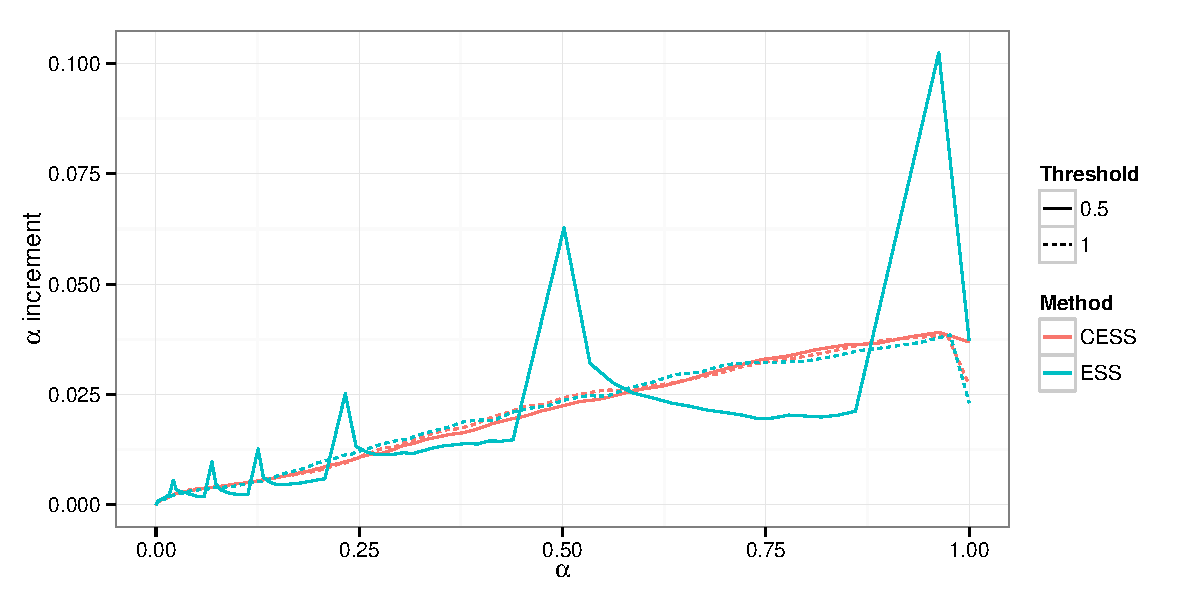
\includegraphics[width=\linewidth]{fig/Adaptive_Dist}
  \caption{A typical plot of $\alpha_t - \alpha_{t-1}$ against $\alpha_t$ (for
    the \pet compartmental model using \smc[2] algorithm.) The specifications of
    the adaptive parameter (\ess or \cess) are adjusted such that all four
    samplers use roughly the same number of distributions.}
  \label{fig:adaptive_alpha}
\end{figure}

More specifically, in practice, when using \cess to adaptively place
distributions, a value $\cess^\star \in (0, 1)$ is chosen, and at each
iteration $t$, $\alpha_t$ is chosen such that $\cess_t = \cess^\star$ (with a
preset numeric error tolerance.) Figure~\ref{fig:adaptive_alpha} shows the
variation of $\alpha_t$ when fixed reductions in \ess and \cess are used to
specify the sequence of distributions both when resampling is conducted during
every iteration (or equivalently, when the $\ess/N$ falls below a threshold of
1.0, where $N$ is the number of particles) and when resampling is conducted
only when the $\ess/N$ falls below a threshold of 0.5. It is found that for
the simulated \pet data set, the \cess-based scheme leads to a reduction in
estimator variance around 20\% relative to a manually tuned ($\alpha(t/T) =
(t/T)^5$) schedule while the \ess-based strategy provides little improvement
over the linear case ($\alpha(t/T) = t/T$) unless resampling is conducted
during every iteration. The effect for the real data sets, which varies
considerably from each as seen in figure~\ref{fig:typical real pet}, is more
prominent. The variance reduction can more than 50\%. More performance
comparisons for various settings of the samplers can be found in
section~\ref{sub:Nonlinear ordinary differential equations}
and~\ref{sub:Positron Emission Tomography compartmental model}.

\subsubsection[cess*, number of distributions, and estimator variance]
{$\cess^\star$, number of distributions, and estimator variance}
\label{ssub:cess*, number of distributions, and estimator variance}

It is intuitively to see that, when using a \cess-based adaptive scheme, where
at each iteration $t$, $\cess_t$ is fixed with a value $\cess^\star$, the more
close $\cess^\star/N$ is to $1$, the larger number of distributions will be placed
and better estimates can be obtained. Unfortunately it is not trivial to
establish a quantitative relations among these three quantities even
asymptotically. However, it is straightforward to conduct an empirical study
of these relations.

We consider the simulated \pet data set using the \smc[2] sampler with 1,000
particles. Figure~\ref{fig:cess iter mean} plots the average number of
distributions (from 100 simulations for each value of $\cess^\star$) against the
value of $(1 - \cess^\star/N)$ on log scales. It can be seen that the number of
distributions is proposal to $(1 - \cess^\star/N)^{-1}$. This relation holds even
for sampler configurations where a very small number of distributions are
used. Similarly, figure~\ref{fig:cess path var} shows the relation between
the variance of path sampling estimator and the value of $\cess^\star$.

\begin{figure}[t]
  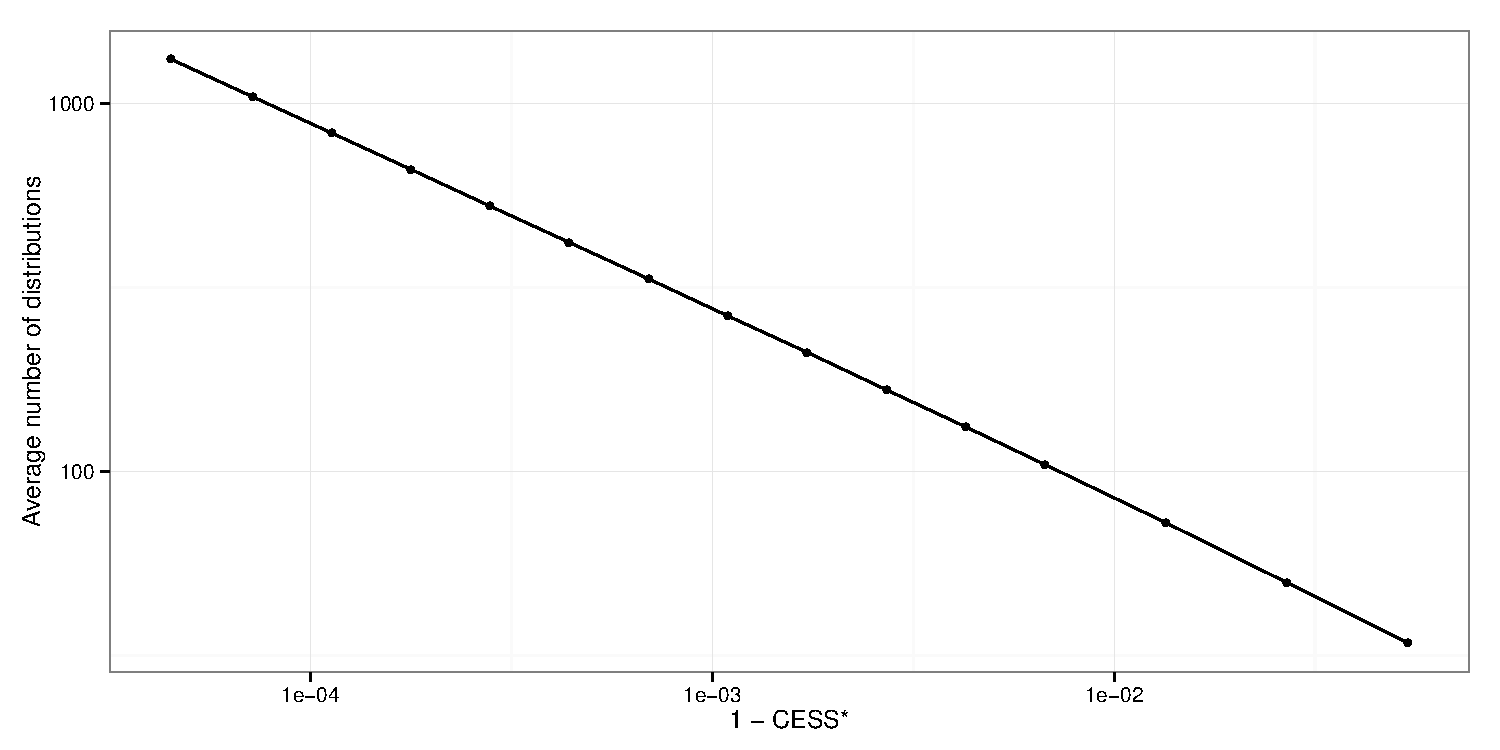
\includegraphics[width=\linewidth]{fig/CESS_Iter_Mean}
  \caption{Relations between average number of distributions and
    $\cess^\star$. The number of distributions ranges from $\sim$30 to
    $\sim$1,300.}
  \label{fig:cess iter mean}
\end{figure}

\begin{figure}[t]
  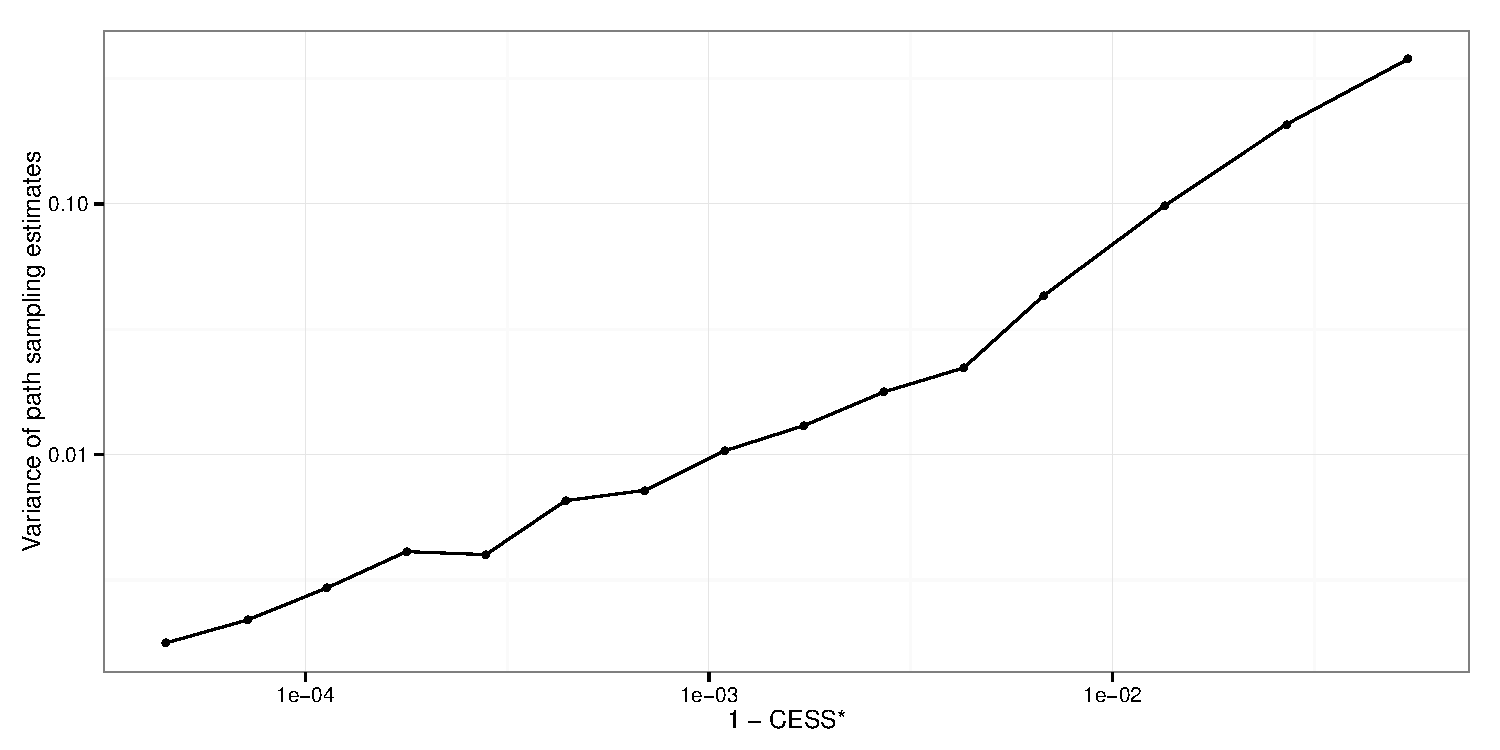
\includegraphics[width=\linewidth]{fig/CESS_Path_Var}
  \caption{Relations between variance of the path sampling estimator and
    $\cess^\star$.}
  \label{fig:cess path var}
\end{figure}

Though the coefficient of the proportionality varies for different
applications or data sets, the relation shown in figures~\ref{fig:cess iter
  mean} and~\ref{fig:cess path var} provide a useful guidelines to select the
value of $\cess^\star$. A small sample experiment can be conducted before using a
value of $\cess^\star$ more close to $1$ to obtain satisfactory estimates or to
utilize given computational resources.

%% \ess only measures the performance of the particle system approximating the
%% target distributions, rather than the variances of the target distributions
%% themselves, which contributes to the variance of incremental weights. As seen
%% in equation~\eqref{eq:smc2-ds} and also for path sampling estimates when using
%% a geometric schedule, the variance of the incremental weights affect the
%% normalizing constants estimates directly. In the case of resampling at every
%% time step, the weights are directly normalized from the incremental weights.
%% In the general situation, as usual, let $W_{n-1}^{(i)}$ denote the
%% \emph{normalized weights} of particle $i$ at the end of time $t = n - 1$, and
%% $w_n^{(i)}$ denote the \emph{unnormalized} incremental weights of particle $i$
%% during the move at $t = n$. In the absence of resampling, we have the
%% recursive relationship,
%% \begin{equation*}
%%   W_n^{(i)} =
%%   \frac{W_{n-1}^{(i)}w_n^{(i)}}{\sum_{j=1}^NW_{n-1}^{(j)}w_n^{(j)}}
%% \end{equation*}
%% and the $\ess_n$,
%% \begin{equation}
%%   \ess_n = \frac
%%   {\bigl(\sum_{j=1}^NW_{n-1}^{(j)}w_n^{(j)}\bigr)^2}
%%   {\sum_{j=1}^N\bigl(W_{n-1}^{(j)}\bigr)^2\bigl(w_n^{(j)}\bigr)^2}
%% \end{equation}
%% If we do resampling after time $t = n - 1$ and before $t = n$, and let
%% $\bar{w}_n^{(i)}$ denote the new incremental weights after resampling, then we
%% have the new $\ess_n$, during move at $t = n$, as,
%% \begin{equation}
%%   \overline{\ess}_n = N \frac
%%   {\bigl(\sum_{j=1}^N\frac{1}{N}\bar{w}_n^{(j)}\bigr)^2}
%%   {\sum_{j=1}^N\frac{1}{N}\bigl(\bar{w}_n^{(j)}\bigr)^2}
%%   \label{eq:ess_before_res}
%% \end{equation}
%% \ess also provides information on ``smoothness'' of the sequence of
%% distributions in the sense that, it measures the discrepancy between sampling
%% distribution and the target distribution and if the target distributions
%% changes little, so shall be \ess. However, this link between \ess and the
%% ``smoothness'' is less direct. Another undesirable aspects of \ess is that its
%% evolution changes when different resampling strategies are used even when the
%% underlying target distributions are the same. Our motivation of extending the
%% concept of \ess is to adaptively place the distributions as if we do
%% resampling at every step without actually carrying out the resampling. Using
%% the unbiasedness of resampling, we can approximate $\overline{\ess}_n$ with
%% \begin{equation}
%%   \cess_n = \frac
%%   {\bigl(\sum_{j=1}^NW_{n-1}^{(j)}w_n^{(j)}\bigr)^2}
%%   {\sum_{j=1}^N\frac{1}{N}W_{n-1}^{(j)}\bigl(w_n^{(j)}\bigr)^2}
%% \end{equation}
%% where by $\cess_n$ we denote the ``conditional \ess'' as it depends upon a
%% consistent approximation of the variance of incremental weights. If we have
%% independent, identically distributed samples from the target distribution at
%% time $t = n - 1$, then $\cess_n$ tells us, essentially, how much variability
%% there would be in those incremental weights. And this variability reflects the
%% difference of the target distribution at time $t = n$ with the previous one.
%% This link is more obvious in the case where
%% equation~\eqref{eq:inc weight mcmc} is used to calculate the incremental
%% weights $w_n(x_{n-1},x_{n}$). Intuitively, \cess provides a direct measurement
%% of the ``smoothness'' of the sequence of distributions.

%% When resampling is performed at every step, then $\cess_n = \ess_n$.
%% Asymptotically, as the number of particles goes to infinity, adaptively
%% placing distributions such that $\cess_n = \cess^\star$ for a fixed value
%% $\cess^\star$ will give the same schedule as the resampling-every-time \ess
%% variant.

\subsection{Adaptive specification of proposals}
\label{sub:Adaptive specification of proposals}

The \smc sampler is remarkably robust to the mixing speed of \mcmc kernels
employed as can be seen in the empirical study below. However, as with any
sampling algorithms, faster mixing doesn't harm performance and in some cases
will considerably improve it. In the particular case of Metropolis-Hastings
kernels, the mixing speed relies on adequate proposal scales.

We adopt a simpler approach based on \cite{Jasra:2010eh}. They applied an idea
used within adaptive \mcmc methods \cite{Andrieu:2006tw} to \smc samplers by
using variance of parameters estimated from its particle system approximation
as the proposal scale for the next iteration, suitably scaled with reference
to the dimension of the parameters to be proposed. Although, in practice we
found that such an automatic approach does not always lead to optimal accept
rates it generally produces satisfactory results and is simple to implement.
In difficult problems alternative approaches to adaptation could be employed;
one approach demonstrated in \cite{Jasra:2010eh} is to simply employ a pair of
accept rate  thresholds and to alter the proposal scale from the simply
estimated value whenever the accept rate falls outside those threshold values.

More sophisticated proposal strategies could undoubtedly improve performance
further and warrant further investigation. One possible approach is using the
Metropolis adjusted Langevin algorithm (\mala; see \cite{Roberts:1996vd}.) In
summary, \mala derives a Metropolis-Hastings proposal kernel for a target
$\pi$ which satisfies suitable differentiability and positivity conditions,
from the Langevin diffusion,
\begin{equation*}
  \diff L_t = \frac{1}{2}\nabla\log\pi(L_t)\diff t + \diff B_t
\end{equation*}
where $B_t$ is the standard Brownian motion. Given a state $X_{n-1}$, a new
state is proposed by discrete approximation to the above diffusion. That is,
for a fixed $h>0$,
\begin{equation}
  X_n\sim\calN\Bigl(X_{n-1}+\frac{1}{2}\nabla\log\pi(X_{n-1}), hI_d\Bigr)
\end{equation}
where $I_d$ is the identify matrix and $d$ is the dimension of the state
space. The new proposed state is accepted or rejected through the usual
Metropolis-Hastings algorithm. Compared to a ``vanilla'' random walk, which
often has very robust theoretical properties, \mala is attractive when it is
possible and its convergence conditions \cite{Roberts:1996vd} can be met,
because only one discrete approximation parameter $h$ needs to be tuned
for optimal performance. In addition, results from \cite{Roberts:2001ta}
suggested that \mala can be more efficient than a random walk when using
optimal scalings. We could also use the particle approximation at time index
$t = n - 1$ to estimate the covariance matrix of $\pi_{n}$ and thus tune the
scale $h$ on-line. As these algorithms are known to be somewhat sensitive to
scaling, and we seek approaches robust enough to employ with little user
intervention, we have not investigated this strategy here.

\begin{figure}[t]
  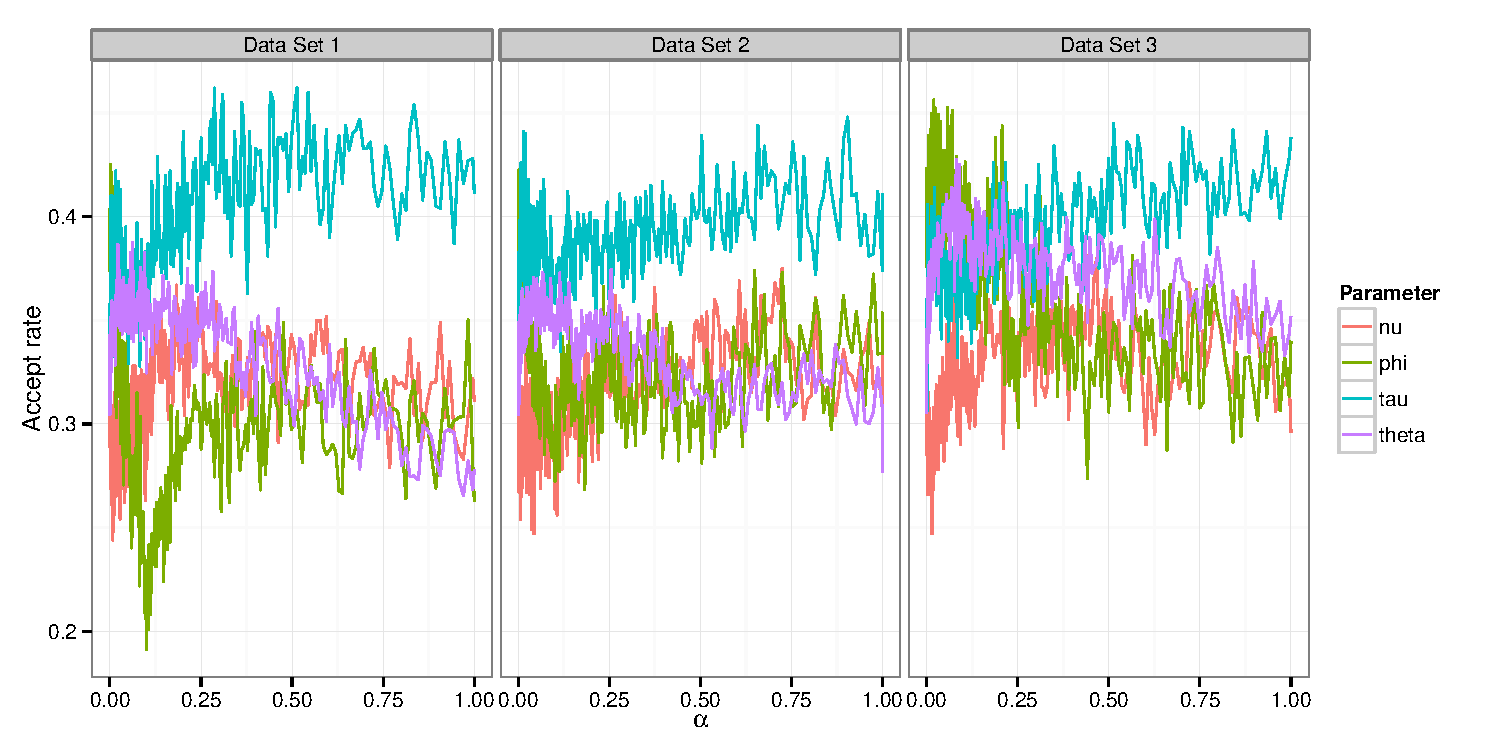
\includegraphics[width=\linewidth]{fig/Adaptive_Proposal}
  \caption{Average random walk accept rates for \pet compartmental models with
    data sets in figure~\ref{fig:typical real pet} using adaptive
    proposal scales}
  \label{fig:pet adaptive proposal}
\end{figure}

\begin{figure}[t]
  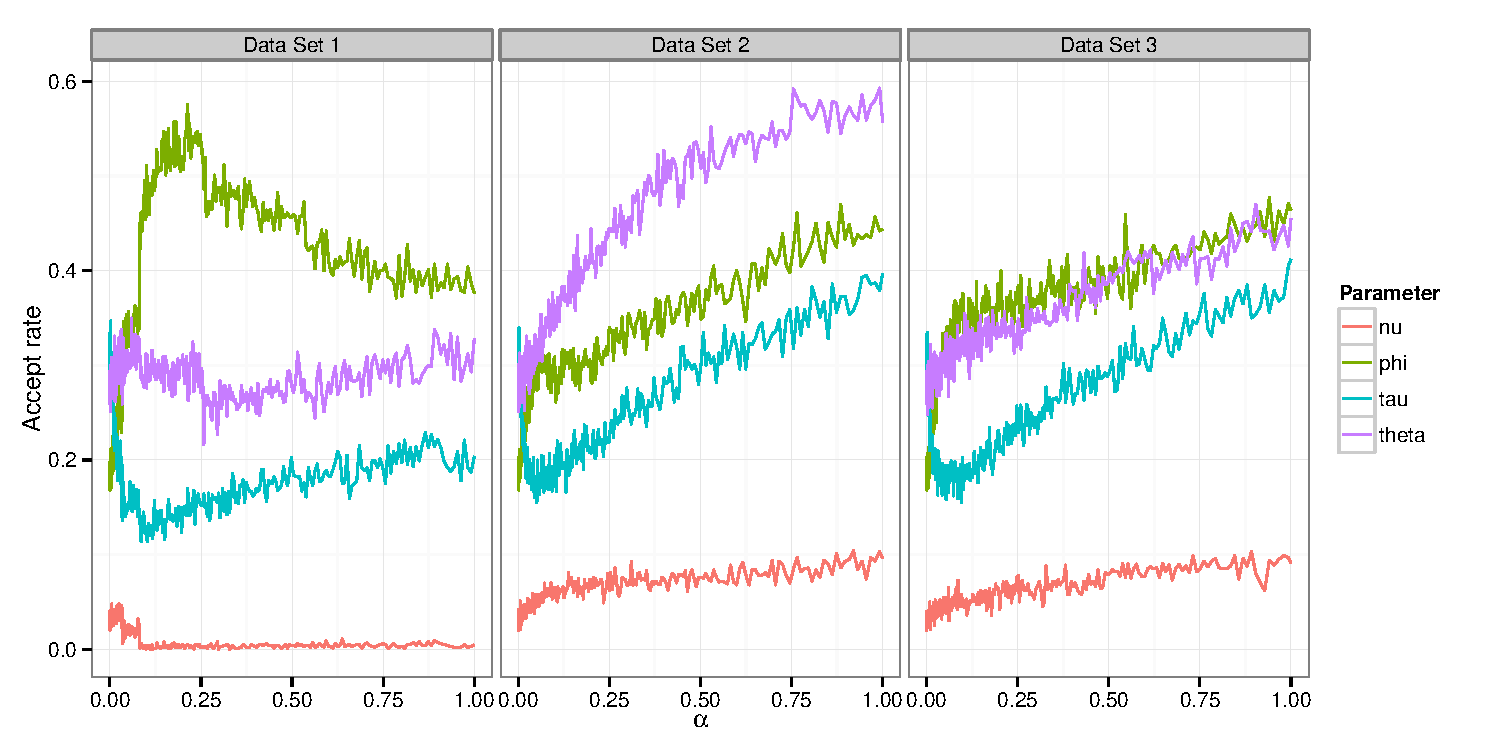
\includegraphics[width=\linewidth]{fig/Fixed_Proposal}
  \caption{Average random walk accept rates for \pet compartmental models with
    data sets in figure~\ref{fig:typical real pet} using fixed proposal
    scales}
  \label{fig:pet fixed proposal}
\end{figure}

Adaptive specification of proposals is most useful when manual tuning is
difficult or even impossible. We consider the three real \pet data sets shown
in figure~\ref{fig:typical real pet}. When using adaptive proposal scales, the
average accept rates of the four random walk blocks (for parameters
$\phi_{1:r}$, $\theta_{1:r}$, $\tau$ and $\nu$, respectively), is shown in
figure~\ref{fig:pet adaptive proposal}. Though the results are not close to
the optimal value $0.234$, which is commonly used in practice, they are more
than acceptable. In contrast, in figure~\ref{fig:pet fixed proposal} we show
the average accept rates when using a scheme of proposal scales which is
obtained from another typical real \pet data set. The scheme is tuned such
that for all parameters, the accept rates falls within the range $[0.2, 0.4]$
for $\alpha_t \in [0, 1]$. It can be seen that, not only the results varies
considerably due to the variety of the data sets, which is expected, for one
of the data set, the parameter $\nu$ fails to move at all. Considering that
there are about a quarter million such data sets to be estimated in a single
\pet scan, adaptively specifying the proposal scales is the only vital
approach. Note that, this problem is not unique to the \pet compartmental
models at all. In many realistic applications, there are a large number of
data sets varies considerably from each other.

%A simpler alternative is based on the observation that in many situations,
%especially in Bayesian model comparison context (for example using a \smc[2]
%sampler for computing model evidences), the sampler starts with a distribution
%(e.g., the prior) whose parameters have large variances and moves towards a
%highly concentrated distribution (e.g., the posterior). Therefore it is
%sensible to have the proposal scales decays sequentially. One scheme to
%construct such a decay is having the proposal scale, say $\sigma$ decays in
%such a form $\sigma = \sigma^\star(b / (a + b\alpha))^p$ where $\sigma^\star$, $a$,
%$b$ and $p$ are constants controlling the speed of and end points of the decay
%and $\alpha$ is the schedule parameter which lies in $[0,1]$ (e.g., the
%$\alpha(t/T)$ in the previous geometric annealing scheme). The constants shall
%be chosen such that the accept rates of the random walk are controlled in an
%acceptable range for all distributions. Practically, one can afford using a
%relatively smaller number of particles and modest number of distributions as a
%pilot run of the algorithm. Using the pilot sampler to tune the constants.
%This simple alternative does indeed require some effort for choosing the
%constants. The benefit is one does not need to tune the proposal scales for
%many iterations, yet avoid the possible situation that with a fully automatic
%adaptation, the accept rates are not always satisfactory.
%
%In the special case of conjugate Normal prior, that is for data $\data$ and a
%parameter of interest $\mu$, $\data|\mu \sim \calN(\mu,\lambda^{-1})$ and
%$\mu \sim \calN(\xi, \kappa^{-1})$ and a geometric annealing scheme, namely
%$\pi_t(\mu)\propto\pi(\mu)[p(\data|\mu)]^{\alpha(t/T)}$, it is well known that
%at time $t$, $\pi_t(\mu)$ is a normal density with variance $(\kappa +
%n\lambda\alpha)^{-1}$ where $n$ is the number of data points. Therefore if we
%follow \cite{Jasra:2010eh} and use the parameter variance as proposal scale,
%the above scheme indeed produce the ``optimal'' scales with the constants
%properly chosen. In more general Bayesian modeling cases, with large amount of
%data, the posterior distribution are asymptotically Normal. This observation
%suggest more general usefulness of the above deterministic scheme. Other
%specification of the decay is also possible. In section~\ref{sec:Illustrative
%  Applications} we demonstrate the effectiveness of this scheme empirically.
%
%Adaptive schemes for either a random walk or an \mala algorithm are
%conceptually appealing and require little computational cost and manual
%tuning. However in practice the results may not be satisfactory and the
%performance can depend on the type of the random walks. In contrast the
%deterministic automatic schemes give users more control of the tuning though
%the choice of the constants may not be obvious in interesting problems.

\section{An automatic, generic framework}
\label{sec:An automatic, generic framework}

With the above refinements, we are ready to implement the \smc[2] algorithm
with minimal tuning and application-specific effort while providing robust and
accurate estimates of the model evidence $p(\data|\Mk)$. First the geometric
annealing scheme that connects the prior $\pi(\paramk|\Mk)$ and the posterior
$\pi(\paramk|\data,\Mk)$, provides a smooth path for a wide range of problems.

Second, the actual annealing schedule under this scheme can be determined
through the adaptive schedule as described above. The advantage of the
adaptive schedule will be shown empirically later.

Third, we can adaptively specify the Metropolis random walk (or \mala) scales
through the estimation of their scaling parameters as the sampler iterates. In
contrast to the \mcmc setting, where such adaptive algorithms will usually
require a burn-in period, which will not be used for further estimation, in
\smc, the variance and covariance estimates come at almost no cost, as all the
samples will later be used for marginal likelihood estimation. Additionally,
adaptation within \smc does not require separate theoretical justification --
something which can significantly complicate the development of effective,
theoretically justified schemes in the \mcmc setting. Alternatively, we can
also specify the proposal scales in a deterministic, but sensible way. Since
\smc algorithms are relatively robust to the change of scales, such
deterministic scales will not require the same degree of tuning as is required
to obtain good performance in \mcmc algorithms.

The adaptive strategy can be applied to both algorithms directly. The
applicability to the \smc[3] algorithm depends on the nature of the sequence
of distributions. We outline the strategy in Algorithm~\ref{alg:adaptive}.

\begin{algorithm}
\begin{algorithmic}
  \tophrule
  \STATE \emph{Accuracy control}
  \STATE\STATESKIP Set constant $\cess^\star\in(0,1)$, using a small pilot
  simulation if necessary.

  \STATE \emph{Initialization:} Set $t\leftarrow0$.
  \STATE\STATESKIP Perform the \emph{Initialization} step
    as in Algorithm~\ref{alg:smc1} or~\ref{alg:smc2}

  \STATE \emph{Iteration:} Set $t\leftarrow t + 1$

  \STATE\STATESKIP \emph{Step size selection}
  \STATE\STATESKIP\STATESKIP Use a binary search %(or other search algorithms)
  to find $\alpha^\star$ such that $\cess_{\alpha^\star} = \cess^\star$
  \STATE\STATESKIP\STATESKIP Set $\alpha_t \leftarrow\alpha^\star$ if
    $\alpha^\star \le 1$, otherwise set $\alpha_t\leftarrow1$

  \STATE\STATESKIP \emph{Proposal scale calibration}
  \STATE\STATESKIP\STATESKIP
  Computing the importance sampling estimates of first two moments of
  parameters.
  \STATE\STATESKIP\STATESKIP
  Set the proposal scale of the Markov proposal $K_t$ with the estimated
  parameter variances.

  \STATE\STATESKIP Perform the \emph{Iteration} step as in
  Algorithm~\ref{alg:smc1} or~\ref{alg:smc2} with the found $\alpha_t$
  and proposal scales.

  \STATE \emph{Repeat} the \emph{Iteration} step %up to $t = T$ (or $T_k$ in the
    %case of Algorithm~\ref{alg:smc2})}
    \emph{until $\alpha_t = 1$} then set $T=t$.
  \bottomhrule
\end{algorithmic}
\caption{An Automatic, Generic Algorithm for Bayesian Model Comparison}
\label{alg:adaptive}
\end{algorithm}

As laid out above, the algorithms require minimal tuning. Its robustness,
accuracy and efficiency will be shown in section~\ref{sec:Performance
  comparison} through comprehensive empirical studies. Here we show some
interesting yet intuitively expected results. We consider the simulated \pet
data set, using a \smc[2] sampler with 1,000 particles. It is already shown
that using either the adaptive specification of distribution placement or the
\mcmc proposal scales can give better results. The combination of the two can
lead to even better results. The use \cess-based schedule scheme will not only
place more distributions where the target distributions changes more rapidly,
but also it will place more distributions where the \mcmc algorithm mixes
slower. To illustrate the idea, we consider four configurations of the
sampler. The proposal scales are specified either adaptively or using a fixed
scheme which is manually tuned. The placement of the distributions is either
\cess-based or using a schedule such that $\alpha(t/T_k) = (t/T_k)^5$.

\begin{table}[t]
  \begin{tabularx}{\linewidth}{lXX}
    \toprule
    & \multicolumn{2}{c}{Proposal scales} \\
    \cmidrule(lr){2-3}
    Schedule & Fixed & Adaptive \\
    \midrule
    Quadratic & $1.6\pm0.27$ & $1.6\pm0.22$ \\
    \cess     & $1.6\pm0.19$ & $1.6\pm0.15$ \\
    \bottomrule
  \end{tabularx}
  \caption{Bayes factor estimates ($\log B_{1,2}\pm\sd$) for the simulated
    \pet data set using \smc[2] algorithm. All four samplers are configured such
    that about 200 distributions are used.}
  \label{tab:pet four sampler same dist}
\end{table}

The results are shown in table~\ref{tab:pet four sampler same dist}. More
comprehensive results can be found in section~\ref{sec:Performance
  comparison}. However, from this particular example, we can see that the
combination of the two adaptive schemes provides superior performance at very
little computation cost. Table~\ref{tab:pet four sampler same iter} shows
actually equivalent results. Instead of fixing the number of distributions, we
configured the samplers such that they all give roughly the same precision of
the estimates. It is rather obvious to see that the use of adaptive methods
actually give a considerable reduction of computational cost for a given
desired precision of the estimates.

\begin{table}[t]
  \begin{tabularx}{\linewidth}{lXX}
    \toprule
    & \multicolumn{2}{c}{Proposal scales} \\
    \cmidrule(lr){2-3}
    Schedule & Fixed & Adaptive \\
    \midrule
    Quadratic & $200$ & $182$ \\
    \cess     & $175$ & $157$ \\
    \bottomrule
  \end{tabularx}
  \caption{Number of distributions used for the simulated \pet data set using
    \smc[2] algorithm. All four samplers are configured such that the Bayes
    factor estimates ($\log B_{1,2}$) have a standard deviation $0.27$.}
  \label{tab:pet four sampler same iter}
\end{table}

We shall also note that \smc[1] is less straightforward as the between model
moves still require effort to design and implement. In \smc[3], the
specification of the sequences between posterior distributions are less
generic compared to the geometric annealing scheme in \smc[2]. However, the
adaptive schedule and automatic tuning of \mcmc proposal scales, both can be
applied in these two algorithms in principal.

Although further enhancements and refinements are clearly possible, we focus
in the remainder of this article on this simple, generic algorithm which can
be easily implemented in any application and has proved sufficiently powerful
to provide good estimation in the examples we have encountered thus far.

\section{Theoretical considerations}
\label{sec:Theoretical considerations}

The convergence results for the standard estimator can be found in
\cite{DelMoral:2006hc} and references therein. In this work, given our
advocation of \smc[2]-\ps, we extend the results for the path sampling
estimator from \smc samplers. Here we present Proposition~\ref{prop:path_clt},
which is specific to path sampling estimator using the simplest Trapezoidal
approach to numerical integration. It follows as a simple corollary to a more
general result given in section~\ref{sub:proof of proposition 1} which could
be used to characterize more general numerical integration schemes.

%% Before we present the proposition, we formalize some notations, which follow
%% \cite{DelMoral:2004ux}, where more detailed theoretical treatment of the
%% topic can be found. The importance sampling estimates from a \smc sampler can
%% be viewed as empirical approximation to a Feynman-Kac flow,
%% $\{\hat\eta_t\}_{t\ge0}$, on increasing spaces of
%% $\{E_t^\prime =\prod_{k=0}^tE_k\}_{t\ge0}$. At each iteration $t = n$, the sampling
%% step, which update each particles with a Markov kernel, the distribution
%% $\hat\eta_{n-1}$ is updated with Markov transition $M_n$ to $\eta_n =
%% \hat\eta_{n-1}M_n$, and the resampling step, if multinomial resampling is
%% applied, update the distribution $\eta_n$ to $\hat\eta_n = \Psi_n(\eta_n)$,
%% where
%% \begin{equation}
%%   \Psi_n(\eta_n)(\diff x_{0:n}) =
%%   \frac{G_n(x_{0:n})\eta_n(\diff x_{0:n})}{\eta_n(G_n)}
%% \end{equation}
%% and $G_n(x_{0:n})$ is called the potential function and can be viewed as a
%% generalization of the weighting function before. For example, in the generic
%% algorithm describe in the beginning of Section~\ref{sec:Methodology}, the
%% sequence of distributions on increasing dimensions $\tilde\pi_n$ is
%% interpreted as the flow $\hat\eta_n$. The Markov transition $M_n$ can be
%% defined in terms of the Markov kernel on marginal distributions $K_n(x_{n-1},
%% x_n)$.

%% \comment{Notations are still not quite clear. In the Feynman-Kac
%%   interpretation, actually the $x_n$ here is the path $x_{0:n}$ where the
%%   later $x_n$ is the particle in previous sections. Maybe I shall rewrite this
%%   part in terms of the $x_{0:n}$}{YZ}

%% With a particular \smc algorithm output, $\hat\eta_n$ is approximated by the
%% empirical measure, $\hat\eta_n(\diff x) \approx \frac{1}{N}\sum_{i=1}^N
%% \delta_{X_n^{(i)}}(\diff x)$

%% In the proposition and corollary, we also assume the following regularity
%% conditions on the pair $(G_t, M_t)$,
%% \begin{compactitem}
%%   \item $(G)$ There exists a sequence of strictly positive numbers
%%     $\epsilon_t(G)\in(0,1]$ such that for any $u_t, v_t\in E_t^\prime$,
%%     \begin{equation*}
%%       G(u_t) \ge \epsilon_t(G)G_t(v_t) > 0
%%     \end{equation*}
%%   \item $(M)_m$ There exists some integer $m\ge1$ and some sequence of numbers
%%     $\epsilon_p(M)\in(0,1)$ such that for $p$ and $u_p,v_p\in E_p'$ we have
%%     \begin{equation*}
%%       M_{p,p+m}(u_p,\cdot) = M_{p+1}M_{p+2}\dots M_{p+m}(u_p,\cdot)
%%       \ge \epsilon_p(M) M_{p,p+m}(v_p,\cdot)
%%     \end{equation*}
%% \end{compactitem}

\begin{proposition}\label{prop:path_clt}
  Under the same regularity conditions as are required for the central limit
  theorem given in \cite{DelMoral:2006hc} to hold, given a \smc sampler that
  iterates over a sequence of distributions $\{\pi_t =
  q_{\alpha_t}/Z_{\alpha_t}\}_{t=0}^T$ and applies multinomial resampling at
  each iteration, the path sampling estimator, $\hat\Xi_{T}^{N}$, as
  defined in Equation~\eqref{eq:path_est} obeys a central limit theorem in the
  following sense: Let $\xi_t(\cdot) = \rnd{\log
    q_{\alpha}(\cdot)}{\alpha}\Bigm|_{\alpha = \alpha_t}$, $\beta_{0} =
  \alpha_0 / 2$, $\beta_{T} = \alpha_T / 2$ and for $t \in \{1,\ldots,T-1\}$
  $\beta_t = (\alpha_{t + 1} - \alpha_{t-1})/2$, then, provided $\xi_t$ is
  bounded:
  \begin{equation}
    \lim_{N\to\infty}\sqrt{N}(\hat\Xi_{T}^{N} - \Xi_T)
    \xrightarrow{D}\calN(0, V_T(\xi_{0:T}))
  \end{equation}
  where $V_t$, $0\le t \le T$ is defined by the following recursion:
  \begin{align}
    V_0(\xi_0) =&  \beta_0^2
    \int \pi_0(x_0) (\xi_0(x_0)
    - \pi_0(\xi_0))^2 dx_0 \\
    V_t(\xi_{0:t}) =& V_{t-1}\biggl(\xi_{0:t-2}, \xi_{t-1}
    + \frac{\beta_t}{\beta_{t-1}}
    \frac{\pi_{t}(\cdot)}{\pi_{t-1}(\cdot)}
    \int K_t(\cdot,x_t) (\xi_t(x_t)-\pi_t(\xi_t)) \intd x_t
    \biggr) \\\notag
    &+ \beta_t^2 \int\frac{\pi_t(x_{t-1})^2}{\pi_{t-1}(x_{t-1})}
    K_t(x_{t-1},x_t)(\xi_t(x_t) - \pi_t(\xi_t))^2) \intd x_{t-1} \intd x_t.
  \end{align}

  %% Does anyone have the energy to work out what the /correct/ explicit form is?
  %% With a little effort, the recursion can be explicitly written in the form,
  %% \begin{equation}
  %%   V_T(\xi_{0:T}) = \sum_{j=0}^T\var_{\pi_j}\biggl(
  %%   \sum_{i=j}^T\beta_i\frac{\tilde\pi_{i,j}(X_j)}{\tilde\pi_{j,j}(X_j)}
  %%   \int\tilde\pi_{i|j}(x_i|X_j)(\xi_i(x_i) - \pi_i(\xi_i))\intd x_i
  %%   \biggr)
  %% \end{equation}
  %% where $\tilde{\pi}_{i,j}$ is the $j^{\text{th}}$ coordinate marginal of
  %% $\tilde{\pi}_i$ and we adopt the conventions that $\tilde{\pi}_{j|j}
  %% = \mathsf{Id}$ .

\end{proposition}

Application of similar arguments to those used in \cite{DelMoral:2006hc} to
the historical process associated with the \smc sampler would lead to
essentially the same result, but we find this approach more transparent.  We
note that much recent analysis of \smc algorithms has focused on relaxing the
relatively strong assumptions used in the results upon which this result is
based -- looking at more general resampling schemes \cite{DelMoral:2012jq}
and relaxing compactness assumptions \cite{Whiteley:2013} for example.
However, we feel that this simple result is sufficient to show the
relationship between the path sampling and simple estimators and that in this
instance the relatively simplicity of the resulting expression justifies these
stronger assumptions.

\subsection{Proof of proposition 1}
\label{sub:Proof of proposition 1}

We begin by making some identifications which allow the connection between the
\smc sampler algorithm presented above and Feynman-Kac formula to be made
explicit as the proof relies on approaches pioneered in
\cite{DelMoral:2004ux}. Throughout this appendix we write $\eta K(\cdot) =
\int \eta(dx) K(x,\cdot)$ for any compatible measure $\eta$ and Markov kernel
$K$ and $\eta(\varphi) = \int \eta(dx) \varphi(x)$ for any $\eta$-integrable
function $\varphi$.

A Feynman-Kac formula describes the law of a Markov chain on
$\{(E_t,\mathcal{E}_t)\}_{t\geq 0}$ (with initial distribution
$\hat\eta_0$ and transitions $M_t$) evolving in the presence of a
(time-varying) potential (described by $G_t$) such that the marginal law of
the $t^\text{th}$ coordinate is:
\begin{equation*}
  \hat\eta_t(A) = \frac
  {
    \int_{E_1 \times \ldots \times E_{t-1} \times A}
    \hat\eta_0(d\tilde{x}_0)
    \prod_{i=1}^t M_{i}(\tilde{x}_{i-1},d\tilde{x}_i)
    G(\tilde{x}_i)
  }{
    \int_{E_1 \times \ldots \times E_{t}}
    \hat\eta_0(d\tilde{x}^\prime_0)
    \prod_{i=1}^t M_{i}(\tilde{x}^\prime_{i-1},d\tilde{x}^\prime_i)
    G(\tilde{x}^\prime_i)
  }
\end{equation*}
for any measurable set $A$.

It is convenient to define the operator $\hat\Phi_t(\eta)(\diff
\tilde{x}_t) = G_t(\tilde{x}_t)\eta M_t(\diff \tilde{x}_t)/\eta
M_t(G_t)$ which allows us to write, recursively, $\hat\eta_t =
\hat\Phi_t(\hat\eta_{t-1})$ and to define the intermediate
distributions $\eta_t = \hat\eta_{t-1}M_t$ such that $\hat\eta_t(\diff
\tilde{x}_t) = G_t(\tilde{x}_t) \eta_t(d\tilde{x}_t) /
\eta_t(G_t)$.

If $\mathcal{X}$ denotes the space upon which an \smc sampler with \mcmc
proposal $K_t$ at time $t$ and sequence of target distributions $\pi_t$
operates, then we obtain $\pi_t$ as the final coordinate marginal of the
Feynman-Kac distribution at time $t$ if we identify $E_t = \mathcal{X}^t$,
$M_{t}(\tilde{x}_{t-1},d\tilde{x}_t) =
\delta_{\tilde{x}_{t-1}}(d\tilde{x}_{t,1:t-1})
K_t(\tilde{x}_{t,t-1},d\tilde{x}_t)$ and $G_t(\tilde{x}_t) =
\pi_{t}(\tilde{x}_{t,t-1}) / \pi_{t-1}(\tilde{x}_{t,t-1})$.

To provide symmetry between the simulation system and the ideal system which
it targets, it is convenient to let $\tilde{X}_t^i$ denote the extended
sample corresponding to $X_t^i$ at iteration $t$ together with the full
collection of values which its ancestors took during previous iterations
(i.e., $\tilde{X}_t^i$ corresponds to the particle system obtained by
sampling according to $M_t$ above rather than $K_t$ at each iteration).  It is
then convenient to write the particle approximation at time $t$ as
$$\hat\eta_t^N(d\tilde{x}_t) = \sum_{i=1}^N
\frac{G_t(\tilde{X}_t^i)}{\sum_{j=1}^N G_t(\tilde{X}_t^j)}
\delta_{\tilde{X}_t^i}(d\tilde{x}_t).$$ We refer the reader to
\cite{DelMoral:2004ux} for further details of the connection between such
particle systems and the Feynman-Kac formula.

In order to proceed, we prove the following more general result to which
Proposition~\ref{prop:path_clt} is a direct corollary.

\begin{proposition}\label{prop:gen_clt}
  Under the regularity conditions given in \cite[section 9.4, pp.
  300--306]{DelMoral:2004ux}, a weighted sum of integrals obtained from
  successive generations of the particle approximation of a Feynman-Kac flow
  $\{\hat\eta_t\}_{t=0}^T$, with the application of multinomial resampling
  at every iteration, obeys a central limit theorem in the following sense,
  for a collection of finite weights $\beta_t\in\Real$ and bounded measurable
  functions $\xi_t:E_t \to\Real$ (where, in the historical process case
  described above it is required that $\xi_t(\tilde{x}_t) =
  \xi_t(\tilde{x}_{t,t})$):
  \begin{equation}
    \lim_{N\to\infty}\sqrt{N}
    \sum_{t=0}^T\beta_t(\hat\eta_t^N(\xi_t)-\hat\eta_t(\xi_t))
    \xrightarrow{D}\calN(0,V_T(\xi_{0:T}))
  \end{equation}
  where $V_t$, $0\le t \le T$ is defined by the following recursion:
  \begin{align}
    V_0(\xi_0) =& \beta_0 \int \hat\eta_0(x_0)(\xi_0(x_0) -
    \eta_0(\xi_0))^2 dx_0\notag\\
    V_t(\xi_{0:t}) =& V_{t-1}\biggl(\xi_{0:t-2}, \xi_{t-1}
    + \frac{\beta_t}{\beta_{t-1}}
    \frac{M_t(G_t[\xi_t-\hat\eta_t(\xi_t)])}{\hat\eta_{t-1}M_t(G_t)}\biggr)
    + \beta_t^2\hat\eta_t\left(\frac{G_t(\cdot) (\xi_t(\cdot)-\hat\eta_t(\xi_t))^2}{\hat\eta_t(G_t)}\right).
  \end{align}
\end{proposition}

The strategy of the proof is to decompose the error as that propagated forward
from previous times and that due to sampling at the current time, just as in
\cite{DelMoral:2004ux}.  First note that the term
$\hat\eta_t^N(\xi_t)-\hat\eta_t(\xi_t)$ can be rewritten as
\begin{equation}
  \hat\eta_t^N(\xi_t)-\hat\eta_t(\xi_t) =
  \hat\eta_t^N(\xi_t) - \hat\Phi_t(\hat\eta_{t-1}^N)(\xi_t) +
  \hat\Phi_t(\hat\eta_{t-1}^N)(\xi_t) - \hat\eta_t(\xi_t)
\end{equation}
and the weighted sum,
\begin{equation}
  T_t^N(\xi_{0:t}) =\sqrt{N}
  \sum_{j=0}^t\beta_j(\hat\eta_j^N(\xi_j)-\hat\eta_j(\xi_j))
\end{equation}
can therefore be written as
\begin{align}
  T_t^N(\xi_{0:t}) &= T_{t-1}^N(\xi_{0:t-1}) +
  \sqrt{N}\beta_t(\hat\eta_t^N(\xi_t)-\hat\eta_t(\xi_t)) \notag\\
  &= \bar{T}_t^N(\xi_{0:t}) + \chi_t^N(\xi_t)
\end{align}
where
\begin{align}
  \bar{T}_t^N(\xi_{0:t}) &= T_{t-1}^N(\xi_{0:t-1}) +
  \sqrt{N}\beta_t(\hat\Phi_t(\hat\eta_{t-1}^N)(\xi_t) - \hat\eta_t(\xi_t))
  \label{eq:bar_t_t} \\
  \chi_t^N(\xi_t) &=
  \sqrt{N}\beta_t(\hat\eta_t^N(\xi_t) - \hat\Phi_t(\eta_{t-1}^N)(\xi_t))
\end{align}

Lemma~\ref{lem:propagation} shows that error propagation leads to controlled
normal errors; Lemma~\ref{lem:sampling} shows that the act of sampling during
each iteration also produces a normally-distributed error and
Lemma~\ref{lem:normality} shows that these two normal errors can be combined
leading by induction to Proposition~\ref{prop:gen_clt}.

\begin{lemma}\label{lem:propagation}
  Under the conditions of Proposition~\ref{prop:gen_clt}, if
  $T_{t-1}^N(\xi_{0:t-1})\xrightarrow{D}\calN(0,V_{t-1}(\xi_{0:t-1}))$, then
  \begin{equation}
    \bar{T}_t^N(\xi_{0:t})\xrightarrow{D}\calN(0, \bar{V}_t(\xi_{0:t}))
  \end{equation}
  where
  \begin{equation}
    \bar{V}_t = V_{t-1}\biggl(\xi_{0:t-2}, \xi_{t-1} +
    \frac{\beta_t}{\beta_{t-1}}
    \frac{M_t(G_t[\xi_t-\hat\eta_t(\xi_t)])}{\hat\eta_{t-1}M_t(G_t)}\biggr).
  \end{equation}
\end{lemma}

\begin{proof}
  We begin by re-expressing the difference of interest in a more convenient form:
  \begin{align}
    \hat\Phi(\hat\eta_{t-1}^N)(\xi_t) - \hat\eta_t(\xi_t)
    &= \frac{1}{\hat\eta_{t-1}^NM_t(G_t)}\{
      \hat\eta_{t-1}^NM_t(G_t\xi_t) -
      \hat\eta_{t-1}^NM_t(G_t)\hat\eta_t(\xi_t)\} \notag\\
    &= \frac{1}{\hat\eta_{t-1}^NM_t(G_t)}
    \{(\hat\eta_{t-1}^N-\hat\eta_{t-1})M_t(G_t[\xi_t-\hat\eta_t(\xi_t)])\}
  \end{align}
where the final equality is a simple consequence of the fact that for any
integrable test function $\varphi$:
\begin{equation*}
\hat\eta_{t-1} M_t (G_t \varphi) = \eta_t(G_t) \hat\eta_t(\varphi) \Rightarrow
\hat\eta_{t-1} M_t (G_t [\xi_t - \hat\eta_t(\xi_t)]) = \eta_t(G_t)
\underset{=0}{\underbrace{\hat\eta_t(\xi_t - \hat\eta_t(\xi_t))}} .
\end{equation*}

Substituting this representation into Equation~\eqref{eq:bar_t_t},
  \begin{align}
    \bar{T}_t^N(\xi_{0:t})
    &= T_{t-1}^N(\xi_{0:t-1}) +
    \frac{\sqrt{N}\beta_t}{\hat\eta_{t-1}^NM_t(G_t)}
    \{(\hat\eta_{t-1}^N-\hat\eta_{t-1})M_t(G_t[\xi_t-\hat\eta_t(\xi_t)])\}
    \notag\\
    &= T_{t-1}^N\biggl(\xi_{0:t-2},
    \xi_{t-1} + \frac{\beta_t}{\beta_{t-1}}
    \frac{M_t(G_t[\xi_t-\hat\eta_t(\xi_t)])}{\hat\eta_{t-1}^NM_t(G_t)}\biggr)
  \end{align}
  The proof is completed by using the result \cite[cf.
  Sec.~7.4.3]{DelMoral:2004ux}, that if $G_t$ is essentially bounded below
  then,
  \begin{equation*}
    \frac{1}{\hat\eta_{t-1}^NM_t(G_t)} \xrightarrow{p}
    \frac{1}{\hat\eta_{t-1}M_t(G_t)}
  \end{equation*}
  together with the induction hypothesis.
\end{proof}

\begin{lemma}\label{lem:sampling}
  Under the conditions of Proposition~\ref{prop:gen_clt},
  \begin{equation}
    \lim_{N\to\infty}\chi_t^N(\xi_t)\xrightarrow{D}\calN(0, \hat{V}_t(\xi_t))
  \end{equation}
  where
  \begin{equation}
    \hat{V}_t(\xi_t) = \beta_t^2\hat\eta_t((\xi_t - \hat\eta_t(\xi_t))^2)
  \end{equation}
\end{lemma}

\begin{proof}
  Consider first the particle system before reweighting with the potential
  function $G_t$:
  \begin{equation}
\sqrt{N}\beta_t
    \sum_{j=1}^N\frac{\xi_t(\tilde{X}_t^{(j)}) - \hat\eta_{t-1}^N M_t(\xi_t)}{N}
    = \sum_{j=1}^NU_{t,j}^N
  \end{equation}
  where $U_{t,j}^N = \frac{\beta_t}{\sqrt{N}}\{\xi_t(\tilde{X}_t^{(j)}) -
    \hat\eta_{t-1}^N M_t(\xi_t)\}$. Define, recursively, the $\sigma$-algebras
    $\calH_t^N = \calH_{t-1}^N \vee
    \sigma(\{\tilde{X}_{t}^{(j)}\}_{j=1}^N)$, $\calH_{t-1} =
    \sigma\left(\cup_{N=0}^\infty \calH_{t-1}^N \right)$ and the increasing (in $j$) sequence of
  $\sigma$-algebras $\calH_{t,j}^N =
  \calH_{t-1}\vee\sigma(\{\tilde{X}_t^{(l)}\}_{l=1}^j)$. It is clear that
  \begin{equation}
    \Exp[U_{t,j}^N|\calH_{t,j-1}^N] = \Exp[U_{t,j}^N|\calH_{t-1}] = 0
  \end{equation}
  and so the sequence $U_{t,j}^N$, $j = 1,\dots,N$ comprises a collection of
  $\calH_{t,j}^N$-martingale increments. Further it can be verified that these
  martingale increments are square integrable,
  \begin{align*}
    \Exp[(U_{t,j}^N)^2|\calH_{t,j-1}^N]
    &= \Exp[(U_{t,j}^N)^2|\calH_{t-1}] \\
    &= \frac{\beta_t^2}{N}\{\hat\eta_{t-1}^N M_t(\xi_t^2) -
      [\hat\eta_{t-1}^N)(\xi_t)]^2\}
    < c_t \frac{\beta_t^2}{N} %\biggl\{
     % R_t\lVert\xi_t\rVert_{\infty}^2 + R_t^2\lVert\xi_t\rVert_{\infty}
     % \biggr\}
  \end{align*}
where $c_t < \infty$ exists by the boundedness of $\xi_t$. The
conditional Linderberg
  condition is also clearly satisfied. %(e.g., see proof of Lemma 7{} in
  %\cite{Johansen:2006iv}).
That is, for any $0 < u\le1$ and $\varepsilon>0$,
  \begin{equation*}
    \lim_{N\to\infty}\sum_{j=1}^{\lfloor Nu\rfloor}
    \Exp[(U_{t,j}^N)^2\bbI_{(\varepsilon,\infty)}(|U_{t,j}^N|)|\calH_{t,j}^N]
    \xrightarrow{P}0.
  \end{equation*}
  Thus we have
  \begin{align*}
    \sum_{j=1}^N\Exp[(U_{t,j}^N)^2|\calH_{t,j-1}^N]
    &= \frac{\beta_t^2}{N}\sum_{j=1}^N
    \{\hat\eta_{t-1}^N M_t(\xi_t^2) - [\hat\eta_{t-1}^N M_t(\xi_t)]^2\} \\
    &= \beta_t^2     \{\hat\eta_{t-1}^N M_t(\xi_t^2) - [\hat\eta_{t-1}^N M_t(\xi_t)]^2\}
  \end{align*}
  and we can invoke the martingale central
  limit theorem \cite[pp.~543]{Shiryaev:1995vp},
  \begin{equation}
    \lim_{N \to\infty}\chi_t^N(\xi_t)%|\calH_{t-1}
    \xrightarrow{D}\calN(0,\check{V}_t(\xi_t))
  \end{equation}
  where the asymptotic variance, $\check{V}_t(\xi_t)$, may be written as the limit
  of the sequence defined by
  \begin{equation}
    \check{V}_t^N(\xi_t) = \beta_t^2 \{\hat\eta_{t-1}^N M_t (\xi_t^2) -
      [\hat\eta_{t-1}^NM_t(\xi_t)]^2\}
  \end{equation}
  and as (again, see \cite[Section 7.4]{DelMoral:2004ux})
  \begin{align*}
    \check{V}_t^N(\xi_t)
    &\xrightarrow{P} \beta_t^2 \{\hat\eta_{t-1}M_t(\xi_t^2) -
      [\hat\eta_{t-1}M_t(\xi_t)]^2\}
  \end{align*}
  the proof is completed using Slutzky's lemma and applying \cite[Lemma A2]{Chopin:2004cn} which
  yields that:
\begin{align*}
\lim_{N \rightarrow \infty} \mathcal{X}_t^N \xrightarrow{D} \calN(0,\hat{V}_t(\xi_t))
\end{align*}
with
\begin{align*}
\hat{V}_t(\xi_t) =
\check{V}_t\left(\frac{G_t(\cdot)}{\hat\eta_{t-1}M_t(G_t)} (\xi_t(\cdot) -
\hat\eta_t(\xi_t)) \right) =
\beta_t^2 \hat\eta_t\left(
\frac{G_t(\cdot)}{\hat\eta_{t-1}M_t(G_t)} (\xi_t(\cdot) -
\hat\eta_t(\xi_t))
\right)
\end{align*}
\end{proof}

\begin{lemma}\label{lem:normality}
  Under conditions of Proposition~\ref{prop:gen_clt}, and the inductive
  assumption of Lemma~\ref{lem:propagation}, $T_t^N(\xi_{0:t})$ is
  asymptotically normal with variance stated as in
  Proposition~\ref{prop:gen_clt}.
\end{lemma}

\begin{proof}
  Consider the characteristic function,
  \begin{align*}
    \varphi(T_t^N(\xi_{0:t}))(s)
    &= \Exp[\exp(isT_t^N(\xi_{0:t}))] \\
    &= \Exp[\exp(is\bar{T}_t^N(\xi_{0:t}))\exp(is\chi_t^N(\xi_t))] \\
    &= \Exp[\exp(is\bar{T}_t^N(\xi_{0:t}))
    \Exp[\exp(is\chi_t^N(\xi_t))|\calH_{t-1}^N]] \\
    &= \Exp[(A_t - \exp(-s^2\hat{V}_t(\xi_t)/2))B_t]
    +\exp(-s^2\hat{V}_t(\xi_t)/2)\Exp[B_t]
  \end{align*}
  where $A_t = \Exp[\exp(is\chi_t^N(\xi_t))|\calH_{t-1}^N]$ and $B_t =
  \exp(is\bar{T}^N(\xi_{0:t}))$. The first term can easily be shown to
  converge a.s. to zero as $N\to\infty$ by the asymptotic normality of
  $\xi_t^N$ and the conditional independence of the particles at iteration $t$
  given $\mathcal{H}_{t-1}^N$.  The second term is the product of two Gaussian
  characteristic functions and thus we have that $T_t^N$ also follows a
  Gaussian distribution (see the argument of \cite{Kuensch:2005} shown in more
  detail in Lemma 10{} in \cite{Johansen:2006iv}, which uses essentially the
  same argument, for details).
\end{proof}

Using Lemma~\ref{lem:propagation} to~\ref{lem:normality}, the proof of
Proposition~\ref{prop:gen_clt} follows by mathematical induction and a trivial
base case (the first iteration is simple importance sampling).

\section{Performance comparison}
\label{sec:Performance comparison}

In this section, we will use three examples to illustrate the algorithms. The
Gaussian mixture model is discussed first, with implementations for all three
\smc algorithms with comparison to \rjmcmc and \pmcmc. It will be shown that
all five algorithms agree on the results while the performance in
terms of Monte Carlo variance varies considerably. It will also be
demonstrated how the adaptive refinements of the algorithms behaves in
practice. We will reach the conclusion that considering ease of
implementation, performance and generality, the \smc[2] algorithm is most
promising among all three strategies.

Then two more realistic examples, a nonlinear \ode model and the \pet
compartmental model are used to study the performance and robustness of
algorithm \smc[2] compared to \ais and \pmcmc. Various configurations of the
algorithms are considered including both sequential and parallelized
implementations.

The \texttt{C++} implementations, which make use of the vSMC library of
\cite{software:VSMC}, of all examples can be found at
\url{https://github.com/zhouyan/vSMC}.

\subsection{Gaussian Mixture Model}
\label{sub:Gaussian Mixture Model}

Since \cite{Richardson:1997ea}, the Gaussian mixture model (\gmm) has
provided a canonical example of a model-order-determination problem. We use
the model formulation of \cite{DelMoral:2006hc} to illustrate the efficiency
and robustness of the methods proposed in this paper compared to other
approaches. The model is as follows; data $\data = (y_1,\dots,y_n)$ are
independently and identically distributed as
\begin{equation*}
  y_i|\theta_r \sim \sum_{j=1}^r \omega_j\calN(\mu_j,\lambda_j^{-1})
\end{equation*}
where $\calN(\mu_j,\lambda_j^{-1})$ denotes the Normal distribution with
mean $\mu_j$ and precision $\lambda_j$; $\theta_r =
(\mu_{1:r},\lambda_{1:r},\omega_{1:r})$ and $r$ is the number of components
in each model. The parameter space is thus $\Real^r \times (\Real^{+})^r\times
\Delta_r$ where $\Delta_r = \{\omega_{1:r}:0\le\omega_j\le1;
\sum_{j=1}^r\omega_j=1\}$ is the standard $r$-simplex. The priors which are
the same for each component are taken to be
$\mu_j\sim\calN(\xi,\kappa^{-1})$, $\lambda_j\sim\calGa(\nu,\chi)$ and
$\omega_{1:r}\sim\calD(\rho)$ where $\calD(\rho)$ is the symmetric Dirichlet
distribution with parameter $\rho$ and $\calGa(\nu,\chi)$ is the Gamma
distribution with shape $\nu$ and scale $\chi$. The prior parameters are set
in the same manner as in \cite{Richardson:1997ea}. Specifically, let $\ymin$
and $\ymax$ be the minimum and maximum of data $\data$, the prior parameters
are set such that
\begin{equation*}
  \xi = (\ymax + \ymin) / 2, \quad \kappa = (\ymax - \ymin)^{-2}, \quad
  \nu = 2, \quad \chi = 50\kappa, \quad \rho = 1
\end{equation*}
The data is simulated from a four components model with $\mu_{1:4} = (-3, 0,3,
6)$, and $\lambda_j =2$, $\omega_j = 0.25$, $j = 1,\dots,4$.

We consider several algorithms. First the \rjmcmc algorithm as in
\cite{Richardson:1997ea}, and second an implementation of the \smc[1]
algorithm. Next \ais, \pmcmc and \smc[2] are used for within-model
simulations. The last is an implementation of the \smc[3] algorithm. In all
the algorithms, the local move which does not change the dimension of the
model is constructed as a composition of Metropolis-Hastings random walk
kernels:
\begin{enumerate}
  \item Update $\mu_{1:r}$ using a multivariate Normal random walk proposal.
  \item Update $\lambda_{1:r}$ using a multivariate Normal random walk on
    logarithmic scale, i.e., on $\log\lambda_{j}$, $j = 1, \dots, r$.
  \item Update $\omega_{1:r}$ using a multivariate Normal random walk on logit
    scale, i.e., on $\omega_{j}/\omega_r$, $j = 1,\dots,r-1$.
\end{enumerate}
The \rjmcmc, \smc[1] and \smc[3] algorithms use two additional
reversible jump moves. The first is a combine and split move; the second is a
birth and death move. Both are constructed in the same manner as in
\cite{Richardson:1997ea}. Also in these implementations, an adjacency
condition was imposed on the means $\mu_{1:r}$, such that $\mu_1 < \mu_2 <
\dots < \mu_r$. No such restriction was used for other algorithms.

In \smc[1], \smc[2] and \pmcmc implementations, the distributions are chosen
with a geometric schedule, i.e., as in Equation~\eqref{eq:geometry_1} for
\smc[1] and Equation~\eqref{eq:geometry_2} for the other two. This annealing
scheme has been used in \cite{DelMoral:2006hc,Jasra:2007in} and many other
works. The geometric scheme can also be seen in \cite{Calderhead:2009bd} for
\pmcmc tempering. A schedule $\alpha(t/T) = (t/T)^p$, with $p = 2$ was used.
The rationale behind this particular schedule can be seen in
\cite{Calderhead:2009bd} and other values of $p$ were also tried while
$p\approx2$ performs best in this particular example. The adaptive schedule
was also implemented for \smc[2] and \ais algorithms.

The proposal scales for each block of the random walks are specified
dynamically according to values of $\alpha(t/T)$ for the \smc[2] and \ais
algorithms and also manually tuned for other algorithms such that the
acceptance rates fall in $[0.2, 0.5]$. Later for the \smc[2] and \ais
algorithms, we also consider adaptive schedule of the distribution
specification parameter $\alpha(t/T)$ and the proposal scales of the random
walks.

For \smc[2], \smc[3] and \ais we consider both the direct estimator and the
path sampling estimator. For \pmcmc we consider the path sampling estimator.

\subsubsection{Results}
\label{sec:gmm_res}

The \smc[1] implementation uses 10,000 particles and 500 distributions. The
\rjmcmc implementation uses five million iterations in addition to one million
iterations of burn-in period. The resulting estimates of model probabilities
are shown in Table~\ref{tab:gmm-prob}.

The \smc[2], \smc[3] and \ais implementations use 1,000 particles and 500
iterations. The \pmcmc implementation uses 50 chains and 10,000 iterations in
addition to 10,000 iterations of burn-in period -- these implementations have
approximately equal computational costs. From the results obtained under the
\smc[1] and \rjmcmc algorithms it is clear that, in this particular example,
simulations for models with fewer than ten components are adequate to
characterize the model space. Therefore, under this configuration, the cost is
roughly the same in terms of computational resources as that of the \smc[1]
and \rjmcmc algorithms. From the results of \rjmcmc and \smc[1], we consider
four and five components models (i.e., the true model and the most competitive
amongst the others.) The estimates are shown in Table~\ref{tab:gmm-pair}
which, like all of the other tables in this section, summarises the Monte
Carlo variability of 100 replicate runs of each algorithm.

\draftnote{There are still some overfull boxes in this
  Table~5.3, but it shall look just fine once I drop the
  draft option of the document class and do not show the overfull bars}

\begin{table}[t]
  \linespread{1.1}\selectfont
  \caption
  [Gaussian mixture model posterior model probability]
  {Gaussian mixture model posterior model probability estimates obtained via
    \smc[1] and \rjmcmc.}
  \label{tab:gmm-prob}
  \begin{tabu}{X[2l]X[2.5l]X[1c]X[1c]X[1c]X[1c]X[1l]X[1c]X[1c]}
    \toprule
    & & \multicolumn{7}{c}{Number of components} \\
    \cmidrule(lr){3-9}
    Quantity & Algorithm & $\le2$ & $3$ & $4$ & $5$ & $6$ & $7$ & $\ge8$ \\
    \midrule
    $\Prob(\calM_k|\data)$ & \smc[1]
    & $0$ & $0.0022$ & $0.89$ & $0.10$ & $0.0064$ & $0.0014$ & $0$ \\
    & \rjmcmc
    & $0$ & $0.0013$ & $0.89$ & $0.10$ & $0.0062$ & $0.0025$ & $0$ \\
    $\log B_{4,k}$     & \smc[1]
    & $\infty$ & $6.00$ & $0$ & $2.15$ & $4.93$ & $6.45$ & $\infty$ \\
    & \rjmcmc
    & $\infty$ & $6.53$ & $0$ & $2.15$ & $4.97$ & $5.87$ & $\infty$ \\
    \bottomrule
  \end{tabu}
\end{table}

\begin{table}
  \begingroup\small\begin{tabularx}{\linewidth}{lRRRRRRR}
    \toprule
    & \multicolumn{7}{c}{Algorithms} \\
    \cmidrule(lr){2-8}
    Quantity
    & \smc[2]-\ds & \smc[2]-\ps & \smc[3]-\ds & \smc[3]-\ps & \ais-\ds & \ais-\ps &
    \pmcmc \\
    \midrule
    $\log B_{4,5}$
    & $2.15$ & $2.15$ & $2.16$ & $2.21$ & $2.16$ & $2.17$ & $2.63$ \\
    \sd
    & $0.25$ & $\color{MRed}{0.22}$
    & $0.61$ & $0.62$ & $1.12$ & $1.10$ & $0.41$ \\
    \bottomrule
  \end{tabularx}\endgroup
  \caption{Gaussian mixture model estimates obtained via \smc[2], \smc[3], \ais
    and \pmcmc}
  \label{tab:gmm-pair}
\end{table}


From Tables~\ref{tab:gmm-prob} and~\ref{tab:gmm-pair}, it can be seen that the
standard estimators (\rjmcmc, \smc[1], \smc[2]-\ds, \smc[3]-\ds and \ais-\ds)
agree with each other. Among the path sampling estimators, \smc[2]-\ps and
\ais-\ps have little bias. \smc[3]-\ps shows a little more bias. The \pmcmc
algorithm has a considerable larger bias as the number of distributions is
relatively small (as noted previously, a larger number will negatively affect
the mixing speed.) In terms of Monte Carlo variance, in
Table~\ref{tab:gmm-pair}, \smc[2] clearly has an advantage compared to its
no-resampling variant, \ais. The differences of Monte Carlo \sd between
\smc[2], \smc[3] and \pmcmc, although they do not affect model selection in
this particular example, are considerable.

\paragraph{Effects of resampling} It is clear from these results that
resampling (when required) can substantially improve the estimation of
normalising constants within an \smc framework. This doesn't contradict the
statement in \cite{DelMoral:2006hc} which suggests that resampling may not
much help when the normalising constant is the object of interest, the
theoretical argument which supports this relies upon the assumption that the
Markov kernel used to mutate the particles mixes extremely rapidly and the
result is obtained under the assumption that resampling is performed after
every iteration. When the Markov kernel is not so rapidly mixing, the
additional stability provided by the resampling operation can outweight the
attendant increase in Monte Carlo variance and that is what we observed here
(and in the case of the other examples considered below; results not shown.)

\begin{figure}
  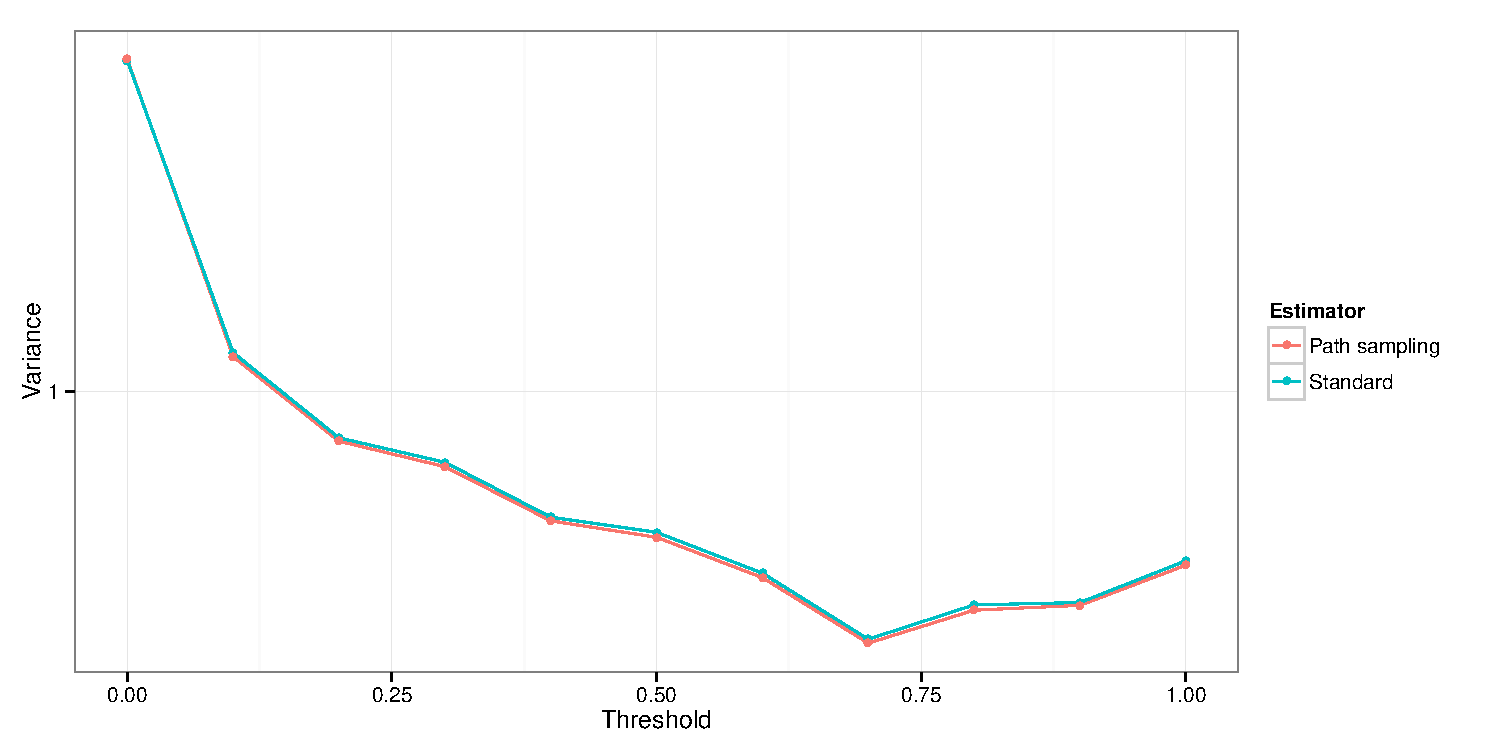
\includegraphics[width=\linewidth]{fig/GMM_Resample}
  \caption{Monte Carlo variance of standard estimator and path sampling
    estimator using different threshold of $\ess/N$ for Gaussian mixture model
    with \smc[2] algorithm. The variance is ploted on log scale}
  \label{fig:gmm resample}
\end{figure}

On the other hand, in this work we advocate resampling adaptively instead of
resampling every iteration. The proposed adaptive schedule also has
significant adavantage in this situation. It is of interest to see if adaptive
resampling has performance improvement when compared to resampling every
iteration. We consider using the \smc[2] algorithm with 1,000 particles, 100
distributions scheduled as $\alpha(t/T) = (t/T)^2$, and various threshold of
$\ess/N$ under which resampling is performed. The Monte Carlo variance of both
the standard estimator and the path sampling estimator is shown in
figure~\ref{fig:gmm resample}. It can be shown that either performing
resampling every iteration or never performing resampling (i.e., \ais), gives
optimal results. Though it may be difficult to determine an optimal value, the
value 0.5 seems to be suitable for this particluar example, as commonly used
in practice.

\paragraph{Effects of adaptive schedules} To assess the evolution of
distributions with an adaptive schedule, we consider the relation between
$\alpha_t - \alpha_{t-1}$ and $\alpha_t$. As stated before, one of the
motivations of using \cess for adaptive placement of distribution is to
ensure that $\alpha_t$ evolves the same path regardless the resampling
strategies. Figure~\ref{fig:adaptive_alpha} shows the evolution of $\alpha_t$
when fixing \ess or \cess and resampling every iteration or only when $\ess <
N/2$. As shown in the plot, when fixing \cess, the evolution of the
distributions is not affected by the resampling strategy. In contrast, fixing
\ess yields a sequence of distributions which depends strongly upon the
resampling strategy.

% Recall that, the purpose of using an adaptive schedule is to construct a
% ``smooth'' sequence of distributions. Though the precise meaning of
% ``smoothness'' may vary from one application to another and both changes in
% \ess and \cess can be reasonably used as measures of it, it shall note that
% at very least, this is a property of the sequence of the distributions
% regardless of the resampling strategies. From this perspective, using is
% \cess is a more plausible approach.

% In terms of the actual performance when using the \cess adaptive strategy
% in \smc[2] algorithm, a reduction of standard deviation of 20\% was
% observed comparing to $\alpha(t/T) = t/T$ and very close to the carefully
% hand-chosen $\alpha(t/T) = (t/T)^2$. When applied to the \smc[3]
% algorithm, 50\% reduction was observed. If the \ess adaptive strategy is
% used instead, similar standard deviation reduction is observed when
% resampling is performed every iteration but no significant effect was
% observed when resampling was only performed when $\ess < N/2$.

In terms of the actual performance when using the \cess adaptive strategy in
the \smc[2] and \ais algorithms, a reduction of standard deviation of 20\% was
observed comparing to $\alpha(t/T) = (t/T)^2$, the one shown in
Table~\ref{tab:gmm-pair}. When applied to the \smc[3] algorithm, 50\%
reduction was observed. If the \ess adaptive strategy is used instead,
similar standard deviation reduction is observed when resampling is performed
every iteration but no significant effect was observed when resampling
was only performed when $\ess < N/2$ (i.e., using \ess rather than \cess
entirely eliminated the benefit.)

\paragraph{Effects of adaptive proposal scales} When using the \smc[2]
algorithm, if the adaptive strategy of \cite{Andrieu:2006tw} is applied,
where the important sampling estimates of the variance of parameters are
included in the adaptation, the acceptance rates fall within $[0.2, 0.5]$
dynamically without manual tuning as for the results in
Table~\ref{tab:gmm-pair}. It should be noted that in this particular example,
it is the variance of $\log\lambda_i$ being estimated as the corresponding
random walk block operates on the log scale. The same principle applies to
the weight parameters, which have random walks on logit scale.
Approximately 20\% reduction in standard deviation was observed.

% However, there are no significant improvement in terms of reduction of
% estimator variances. This can be viewed as evidence that \smc algorithms
% are more robust to the change of proposal scales.

\subsection{Nonlinear ordinary differential equations}
\label{sub:Nonlinear ordinary differential equations}

The example from the previous section suggests that \smc[2] performs well
relative to the other \smc possibilities. Given the wide range of settings
in which it can be easily deployed, we will now concentrate
further on this method. It also suggests that in the simple case of Gaussian
mixtures, a complete adaptive strategy for both distribution specification
and proposal scales works well. In this section, this will now be further
explored in a more complex model, a nonlinear ordinary differential equations
system. This model, which was studied in \cite{Calderhead:2009bd}, is known
as the Goodwin model. The \ode system, for an $m$-component model, is:
\begin{align*}
  \frac{\diff X_1(t)}{\diff t} &= \frac{a_1}{1 + a_2 X_m(t)^{\rho}}
  - \alpha X_1(t)  & \\
  \frac{\diff X_i(t)}{\diff t} &= k_{i-1}X_{i-1}(t) - \alpha X_i(t)
  & i = 2,\dots,m \\
  X_i(0) &= 0 & i = 1,\dots,m
\end{align*}
The parameters $\{\alpha,a_1,a_2,k_{1:m-1}\}$ have common prior distribution
$\calGa(0.1, 0.1)$. Under this setting, $X_{1:m}(t)$ can exhibit either
unstable oscillation or a constant steady state. The data are simulated for
$m=\{3,5\}$ at equally spaced time points from 0 to 60, with time step 0.5.
The last 80 data points of $(X_1(t), X_2(t))$ are used for inference.
Normally-distributed noise with standard  deviation $\sigma=0.2$ is added to
the simulated data. Following \cite{Calderhead:2009bd}, the variance of the
additive measurement error is assumed to be known. Therefore, the posterior
distribution has $m+2$ parameters for an $m$-component model.

As shown in \cite{Calderhead:2009bd}, when $\rho > 8$, due to the possible
instability of the \ode system, the posterior can have a considerable number
of local modes. In this example, we set $\rho = 10$. Also, as the solution to
the \ode system is somewhat unstable, slightly different data can result in
very different posterior distributions.

\subsubsection{Results}

We compare results from the \smc[2] and \pmcmc algorithms. For the \smc
implementation, 1,000 particles and 500 iterations were used, with the
distributions specified specified by Equation~\eqref{eq:geometry_2}, with
$\alpha(t/T) = (t/T)^5$, or via the completely adaptive specification. For
the \pmcmc algorithm, 50,000 iterations are performed for burn-in and another
10,000 iterations are used for inference. The same tempering as was used for
\smc is used here. Note that, in a sequential implementation of \pmcmc, with
each iteration updating one local chain and attempting a global exchange, the
computational cost of after burn-in iterations is roughly the same as the
entire \smc algorithm. In addition, changing $T$ within the range of the
number of cores available does not substantially change the computational cost
of a generic parallel implementation of the \pmcmc algorithm. We compare
results from $T = 10,30,100$.

The results for data generated from the simple model ($m = 3$) and complex
model ($m = 5$), again summarizing variability amongst 100 runs of each
algorithm, are shown in Table~\ref{tab:node-s} and~\ref{tab:node-c},
respectively.

\newgeometry{hmargin={1in,1in},vmargin={1in,2in},bindingoffset=\mclassbinding}

\begin{table}
  \UseAltLinespread
  \caption
  [Nonlinear \protect\ode model marginal likelihood and the Bayes factor
  estimates (simple model data)]
  {Nonlinear \ode model marginal likelihood and the Bayes factor estimates
    with data generated from a simple (three components) model.}
  \label{tab:node-s}
  \begin{tabu}{X[0.3l]X[0.8c]X[0.8c]X[0.8c]X[1r]X[1r]X[1r]}
    \toprule
    &&&& \multicolumn{2}{c}{Marginal likelihood} & Bayes factor \\
    &&&& \multicolumn{2}{c}{$\log p(\data|\calM_k)\pm\sd$} & $\log B_{3,5}\pm\sd$ \\
    \cmidrule(lr){5-6}
    $T$   & Proposal & Annealing & Algorithm   & $r = 3$                & $r = 5$                & \\ \midrule
    $10 $ & Manual         & Prior (5) & \pmcmc      & $-109.7\pm3.2$         & $-120.3\pm2.5$         & $10.6\pm3.8$ \\
    $30 $ &                &           &             & $\SubBest{-105.0\pm1.2}$ & $\SubBest{-116.1\pm2.2}$ & $\SubBest{11.2\pm2.5}$ \\
    $100$ &                &           &             & $-134.7\pm7.9$         & $-144.1\pm6.2$         & $9.4\pm11.2$ \\ \midrule
    $500$ & Manual         & Prior (5) & \smc[2]-\ds & $-104.6\pm2.0$         & $-112.7\pm1.8$         & $8.1\pm2.8$ \\
          &                &           & \smc[2]-\ps & $-104.5\pm1.8$         & $-112.7\pm1.5$         & $8.2\pm2.5$ \\
    $500$ & Manual         & Adaptive  & \smc[2]-\ds & $-104.5\pm1.1$         & $-112.7\pm1.1$         & $8.1\pm1.6$ \\
          &                &           & \smc[2]-\ps & $-104.6\pm1.0$         & $-112.8\pm1.0$         & $8.2\pm1.5$ \\
    $500$ & Adaptive       & Adaptive  & \smc[2]-\ds & $-104.5\pm0.5$         & $-112.7\pm0.4$         & $8.1\pm0.8$ \\
          &                &           & \smc[2]-\ps & $\Best{-104.6\pm0.4}$    & $\Best{-112.8\pm0.3}$    & $\Best{8.1\pm0.6}$ \\
    \bottomrule
    \multicolumn{7}{r}{%
      \begin{minipage}{\linewidth-2em}\vskip1ex\sffamily
        $T$: The number of distributions.

        Proposal: The proposal scales of the \mcmc kernels.

        Annealing: The annealing scheme of the distributions,
        $\alpha_k(t/T_k)$ in Equation~\ref{eq:geometry_2}.

        \Best: The estimate with the smallest variance among all algorithms
        settings.

        \SubBest: The estimate with the smallest variance for a single
        algorithm (\smc[2] or \pmcmc) among different settings.
      \end{minipage}}
  \end{tabu}
\end{table}

\begin{table}
  \UseAltLinespread
  \caption
  [Model selection results of nonlinear \protect\ode model using the Bayes factor (simple model data)]
  {Frequencies of models selected by the Bayes factor (\%) for the nonlinear \ode model with data generated from a simple (three components) model.}
  \label{tab:node-s-mo}
  \begin{tabu}{X[0.3l]X[0.8c]X[0.8c]X[0.8c]X[0.2r]X[0.2r]X[0.2r]X[0.2r]X[0.2r]}
    \toprule
    &&&& \multicolumn{5}{c}{Number of components}\\
    \cmidrule(lr){5-9}
    $T$   & Proposal       & Annealing & Algorithm   & $2$ & $  3$ & $4$ & $5$ & $6$ \\ \midrule
    $10 $ & Manual         & Prior (5) & \pmcmc      & $2$ & $ 96$ & $2$ & $0$ & $0$ \\
    $30 $ &                &           &             & $0$ & $100$ & $0$ & $0$ & $0$ \\
    $100$ &                &           &             & $0$ & $100$ & $0$ & $0$ & $0$ \\
    $500$ & Manual         & Prior (5) & \smc[2]-\ds & $0$ & $100$ & $0$ & $0$ & $0$ \\
          &                &           & \smc[2]-\ps & $0$ & $100$ & $0$ & $0$ & $0$ \\
    $500$ & Manual         & Adaptive  & \smc[2]-\ds & $0$ & $100$ & $0$ & $0$ & $0$ \\
          &                &           & \smc[2]-\ps & $0$ & $100$ & $0$ & $0$ & $0$ \\
    $500$ & Adaptive       & Adaptive  & \smc[2]-\ds & $0$ & $100$ & $0$ & $0$ & $0$ \\
          &                &           & \smc[2]-\ps & $0$ & $100$ & $0$ & $0$ & $0$ \\
    \bottomrule
    \multicolumn{9}{r}{%
      \begin{minipage}{\linewidth-2em}\vskip1ex\sffamily
        $T$: The number of distributions.

        Proposal: The proposal scales of the \mcmc kernels.

        Annealing: The annealing scheme of the distributions,
        $\alpha_k(t/T_k)$ in Equation~\ref{eq:geometry_2}.
      \end{minipage}}
  \end{tabu}
\end{table}

%\restoregeometry

\begin{table}
  \caption{Nonlinear \ode model marginal likelihood and Bayes factor estimates
    with data generated from simple (three components) model.}
  \label{tab:node-c}
  \begin{tabu}{X[1l]X[2c]X[2c]X[2c]X[4r]X[4r]X[6r]}
    \toprule
    &&&& \multicolumn{2}{c}{Marginal likelihood ($\log p(\data|\calM_k)\pm\sd$)} & Bayes factor ($\log B_{3,5}\pm\sd$) \\
    \cmidrule(lr){5-6}
    $T$   & Proposal & Annealing & Algorithm   & $m = 3$                 & $m = 5$                & \\ \midrule
    $10 $ & Manual   & Prior (5) & \pmcmc      & $-1651.0\pm27.9$        & $-85.1\pm36.6$         & $1565.9\pm42.1$ \\
    $30 $ &          &           &             & $\SubBest-1639.7\pm7.4$ & $\SubBest-78.9\pm11.2$ & $\SubBest1560.8\pm12.8$ \\
    $100$ &          &           &             & $-1624.6\pm15.7$        & $-75.7\pm24.8$         & $1548.9\pm25.6$ \\ \midrule
    $500$ & Manual   & Prior (5) & \smc[2]-\ds & $-1640.7\pm10.8$        & $-78.5\pm9.8$          & $1562.2\pm10.1$ \\
          &          &           & \smc[2]-\ps & $-1640.8\pm 8.4$        & $-79.2\pm7.9$          & $1561.6\pm 8.5$ \\
    $500$ & Manual   & Adaptive  & \smc[2]-\ds & $-1639.7\pm 6.9$        & $-78.6\pm4.8$          & $1561.1\pm7.1$ \\
          &          &           & \smc[2]-\ps & $-1640.1\pm 5.4$        & $-78.8\pm3.7$          & $1561.3\pm6.8$ \\
    $500$ & Adaptive & Adaptive  & \smc[2]-\ds & $-1639.8\pm 2.2$        & $-79.4\pm1.7$          & $1560.4\pm3.1$ \\
          &          &           & \smc[2]-\ps & $\Best-1640.2\pm 1.9$   & $\Best-78.5\pm1.5$     & $\Best1561.7\pm2.3$ \\
    \bottomrule
    \multicolumn{7}{r}{%
      \begin{minipage}{\linewidth-2em}\vskip1ex\sffamily
        $T$: The number of distributions. That is, the number parallel \mcmc
        chains for \pmcmc algorithm and the number of iterations for the \smc
        algorithm. For the \pmcmc algorithm, at each iteration, a single \mcmc
        chain is chosen randomly to be updated. There is a 50,000 iterations
        burin period and another 10,000 iterations are used for inference. For
        the \smc algorithm, 1,000 particles are used.

        Proposal: The proposal scales of the \mcmc kernels. The ``Manual''
        proposal is manually tuned such that the accept rates fall between
        $[0.2, 0.6]$. The ``Adaptive'' proposal is dynamically set using
        moments estimates from the last iteration of the particle system.

        Annealing: The annealing scheme of the distributions, $\alpha(t/T_k)$
        in Equation~\ref{eq:geometry_2}. The ``Prior (5)'' scheme is
        concentrated around the prior distribuiton, with $\alpha(t/T_k) =
        (t/T_k)^5$. The ``Adaptive'' scheme set $\alpha$ dynamically such that
        for each iteration, \cess is a constant. The constant value of \cess
        is chosen such that on average, 500 iterations was produced.

        \Best: The estimate with the smallest variance among all algorithms
        settings.

        \SubBest: The estimate with the smallest variance for a single
        algorithm (\smc[2] or \pmcmc) among different settings.
      \end{minipage}}
  \end{tabu}
\end{table}


As shown in both cases, the number of distributions can affect the performance
of \pmcmc algorithms considerably. When using 10 distributions, large bias
from numerical integration for path sampling estimator was observed, as
expected. With 30 distributions, the performance is comparable to the \smc[2]
sampler, though some bias is still observable. With 100 distributions, there
is a much larger variance because, with more chains, the information travels
more slowly from rapidly mixing chains to slowly mixing ones and consequently
the mixing of the overall system is inhibited.

The \smc algorithm provides results comparable to the best of
three \pmcmc implementations in essentially all settings, including one in
which both the annealing schedule and proposal scaling were fully
automatic. In fact, the completely adaptive strategy was the most successful.

It can be seen that increasing the number of distributions not only reduces
the bias of numerical integration for path sampling estimator, but also
reduces the variance considerably. On the other hand increasing the number of
particles can only reduce the variance of the estimates, in accordance with
the central limit theorem (see \cite{DelMoral:2006hc} for the standard
estimator and extensions for path sampling estimator,
Proposition~\ref{prop:path_clt}) (as the bias arises from the numerical
integration scheme.) Therefore, though there exists the trade-off between the
number of particles and the number distributions, increasing either of them
can always benefit the accuracy of the estimators. We will study this
trade-off more carefully with the next more realistic example.

\subsection{Positron Emission Tomography compartmental model}
\label{sub:Positron Emission Tomography compartmental model}

It is now interesting to compare the proposed algorithm with other
state-of-art algorithms using the more realistic \pet compartmental model
example.

\begin{figure}[t]
  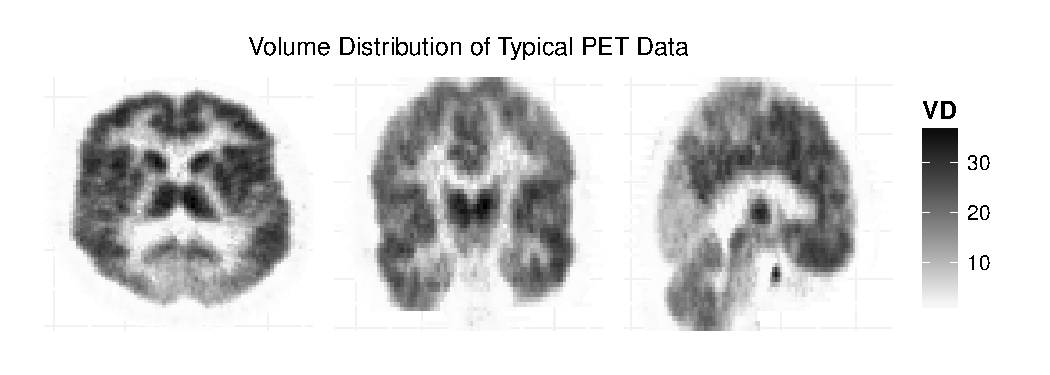
\includegraphics[width=\linewidth]{fig/PETPlot-smc2-ps-bw}
  \caption{Estimates of $V_D$ from a single \pet scan as found using \smc[2].
    The data shows that the volume of distribution exhibits substantial
    spatial variation. Note that each pixel in the image represent an estimate
    from an individual time series data set. There are approximately a quarter
    million of them and each requires a Monte Carlo simulation to select a
    model.}
  \label{fig:petplot}
\end{figure}

As mentioned before, real neuroscience data sets involve a very large number
($\sim$200,000 per brain) of time series, which are typically somewhat
heterogeneous (also see figure~\ref{fig:typical real pet}.)
Figure~\ref{fig:petplot} shows estimates of $V_D$ from a typical \pet scan
generated using \smc[2] as will be discussed later. Robustness is therefore
especially important. An application-specific \mcmc algorithm was developed
for this problem in \cite{Zhou2013} and its results is shown in the last
chapter. A significant amount of tuning of the algorithms was required to
obtain good results.The results shown in Figure~\ref{fig:petplot} are very
close to those of \cite{Zhou2013} but, as is shown later, they were obtained
with almost no manual tuning effort and at similar computational cost.

For \smc and \pmcmc algorithms, the requirement of robustness means that the
algorithm must be able to calibrate itself automatically to different data
(and thus different posterior surfaces.) A sequence of distributions which
performs well for one time series may not perform even adequately for another
series. Specification of proposal scales that produces fast-mixing kernels for
one data series may lead to slow mixing for another (as we already see in
section~\ref{sub:Adaptive specification of proposals}.) In the following
experiment, we will use the simulated data set, and choose schedules that
perform both well and poorly for this particular time series. The objective is
to see if the algorithm can recover from a relatively poorly specified
schedule and obtain reasonably accurate results.

\subsubsection{Results}

In this example we focus on the comparison between \smc[2] and \pmcmc. We also
consider parallelized implementations of algorithms. In this case, due to its
relatively small number of chains, \pmcmc can be parallelized completely (and
often cannot fully utilize the hardware capability if a na\"\i ve approach to
parallelization is taken; while we appreciate that more sophisticated
parallelization strategies are possible, these depend instrinsicially upon the
model under investigation and the hardware employed and given our focus on
automatic and general algorithms, we don't consider such strategies here.) The
\pmcmc algorithm under this setting is implemented such that each chain is
updated at each iteration. Further, for the \smc algorithms, we consider two
cases. In the first we can parallelize the algorithm completely (in the sense
that each core has a single particle associated with it.) In this setting we
use a relatively small number of particles and a larger number of time steps.
In the second, we need a few passes to process a large number of particles at
each time step, and accordingly we use fewer time steps to maintain the same
total computation time. These two settings allow us to investigate the
trade-off between the number of particles and time steps. In both
implementations, we consider three schedules, $\alpha(t/T) = t/T$ (linear),
$\alpha(t/T) = (t/T)^5$ (prior), and $\alpha(t/T) = 1 - (1 - t/T)^5$
(posterior). In addition, the adaptive schedule based upon \cess is also
implemented for the \smc[2] algorithm.

Results from 100 replicate runs of the two algorithms under various regimes
can be found in Table~\ref{tab:pet-py} and~\ref{tab:pet-bf} for the marginal
likelihood and Bayes factor estimates, respectively. The \smc algorithms
consistently outperforms the \pmcmc algorithms in the parallel settings. The
Monte Carlo \sd of \smc algorithms is typically of the order of one fifth of
the corresponding estimates from \pmcmc in most scenarios. In some settings
with the smaller number of samples, the two algorithms can be comparable. Also
at the lowest computational costs, the samplers with more time steps and fewer
particles outperform those with the converse configuration by a fairly large
margin in terms of estimator variance. It shows that with limited resources,
ensuring the similarity of consecutive distributions, and thus good mixing,
can be more beneficial than a larger number of particles. However, when the
computational budget is increased, the difference becomes negligible.

\begin{table}
  \def\B{\color{MBlue}\it}
  \def\R{\color{MRed}\bf}
  \begingroup\small
    \begin{tabularx}{\linewidth}{lllCCCC}
      \toprule
      \multicolumn{3}{l}{Proposal scales}  & \multicolumn{3}{c}{Manual} & Adaptive \\
      \cmidrule(lr){1-3}\cmidrule(lr){4-6}\cmidrule(lr){7-7}
      \multicolumn{3}{l}{Annealing scheme} & Prior (5) & Posterior (5) & \multicolumn{2}{c}{Adaptive} \\
      \cmidrule(lr){1-3}\cmidrule(lr){4-4}\cmidrule(lr){5-5}\cmidrule(lr){6-7}
      %
      $T$    & $N$   & Algorithm   & \multicolumn{4}{c}{Marginal likelihood estimates ($\log p(\paramk|\data)\pm\text{\sd}$)} \\ \midrule
      $500$  & $30 $ & \pmcmc      & $ -39.1\pm  0.56$ & $-926.8\pm376.99$ && \\
      $500$  & $192$ & \smc2-\ds & $\B-39.2\pm0.25$ & $\B-39.7\pm1.06$ & $\B-39.2\pm0.18$ & $\R-39.1\pm0.12$ \\
             &       & \smc2-\ps & $\B-39.2\pm0.25$ & $-91.3\pm21.69$  & $\B-39.2\pm0.18$ & $-39.1\pm0.13$   \\
      $100 $ & $960$ & \smc2-\ds & $-39.3\pm0.36$   & $-40.6\pm1.41$   & $-39.2\pm0.31$   & $-39.2\pm0.19$   \\
             &       & \smc2-\ps & $-39.3\pm0.35$   & $302.1\pm46.29$  & $-39.3\pm0.31$   & $-39.2\pm0.18$   \\ \midrule
      $1000$ & $30 $ & \pmcmc      & $ -39.3\pm  0.46$ & $-884.1\pm307.88$ && \\
      $1000$ & $192$ & \smc2-\ds & $\B-39.2\pm0.19$ & $\B-39.4\pm0.68$ & $\B-39.2\pm0.17$ & $\R-39.1\pm0.10$ \\
             &       & \smc2-\ps & $\B-39.2\pm0.19$ & $-66.0\pm13.26$  & $\B-39.2\pm0.17$ & $\R-39.1\pm0.10$  \\
      $200 $ & $960$ & \smc2-\ds & $-39.2\pm0.22$   & $-39.8\pm1.21$   & $-39.2\pm0.18$   & $-39.1\pm0.11$   \\
             &       & \smc2-\ps & $-39.2\pm0.22$   & $175.5\pm26.84$  & $-39.2\pm0.18$   & $-39.2\pm0.11$   \\ \midrule
      $2000$ & $30 $ & \pmcmc      & $ -39.3\pm  0.28$ & $-928.7\pm204.93$ && \\
      $2000$ & $192$ & \smc2-\ds & $-39.2\pm0.14$   & $\B-39.3\pm0.41$ & $-39.1\pm0.12$   & $-39.1\pm0.07$  \\
             &       & \smc2-\ps & $-39.2\pm0.14$   & $-51.2\pm4.30$   & $-39.2\pm0.12$   & $-39.1\pm0.07$  \\
      $400 $ & $960$ & \smc2-\ds & $\B-39.2\pm0.13$ & $-39.4\pm0.73$   & $\B-39.2\pm0.11$ & $-39.2\pm0.07$   \\
             &       & \smc2-\ps & $\B-39.2\pm0.13$ & $106.0\pm14.36$  & $\B-39.2\pm0.11$ & $\R-39.2\pm0.06$ \\ \midrule
      $5000$ & $30$  & \pmcmc      & $ -39.3\pm  0.21$ & $-917.6\pm129.54$ && \\
      $5000$ & $192$ & \smc2-\ds & $-39.2\pm0.09$   & $\B-39.2\pm0.20$ & $-39.2\pm0.08$   & $-39.1\pm0.04$   \\
             &       & \smc2-\ps & $-39.2\pm0.09$   & $-43.8\pm2.13$   & $-39.2\pm0.08$   & $-39.1\pm0.04$   \\
      $1000$ & $960$ & \smc2-\ds & $\B-39.2\pm0.08$ & $-39.2\pm0.31$   & $\B-39.2\pm0.07$ & $\R-39.2\pm0.03$ \\
             &       & \smc2-\ps & $\B-39.2\pm0.08$ & $-65.7\pm5.54$   & $\B-39.2\pm0.07$ & $\R-39.2\pm0.03$ \\
      \bottomrule
    \end{tabularx}
  \endgroup
  \caption{Marginal likelihood estimates of two components \pet model. $T$:
    Number of distributions in \smc and number of iterations used for
    inference in \pmcmc. $N$: Number of particles in \smc and number chains in
    \pmcmc. The \pmcmc and \smc with $N = 192$ are completely $N$-way
    parallelized.  \smc with $N = 960$ are $N/5$-way parallelized. {\B
      Italic}: Minimum variance for the same computational cost and the same proposal
    scales and annealing schemes.  {\R Bold}: Minimum variance for the same computaitonal
    cost and all proposal scales and annealing schemes.}
  \label{tab:pet-py}
\end{table}

% & & $ -39.1\pm  0.56$ & $-926.8\pm376.99$ &&& \\
% & $\B-39.2\pm0.25$ & $\B-39.7\pm1.06$ & $\B-39.2\pm0.18$ & $\R-39.1\pm0.12$ & $\B-39.2\pm0.13$ \\
% & $\B-39.2\pm0.25$ & $-91.3\pm21.69$  & $\B-39.2\pm0.18$ & $-39.1\pm0.13$   & $\B-39.2\pm0.13$ \\
% & $-39.3\pm0.36$   & $-40.6\pm1.41$   & $-39.2\pm0.31$   & $-39.2\pm0.19$   & $-39.2\pm0.18$ \\
% & $-39.3\pm0.35$   & $302.1\pm46.29$  & $-39.3\pm0.31$   & $-39.2\pm0.18$   & $-39.2\pm0.19$ \\ \midrule
% & & $ -39.3\pm  0.46$ & $-884.1\pm307.88$ &&& \\
% & $\B-39.2\pm0.19$ & $\B-39.4\pm0.68$ & $\B-39.2\pm0.17$ & $\R-39.1\pm0.10$ & $-39.2\pm0.11$ \\
% & $\B-39.2\pm0.19$ & $-66.0\pm13.26$  & $\B-39.2\pm0.17$ & $\R-39.1\pm0.10$ & $\R-39.2\pm0.10$ \\
% & $-39.2\pm0.22$   & $-39.8\pm1.21$   & $-39.2\pm0.18$   & $-39.1\pm0.11$   & $-39.2\pm0.11$ \\
% & $-39.2\pm0.22$   & $175.5\pm26.84$  & $-39.2\pm0.18$   & $-39.2\pm0.11$   & $-39.2\pm0.12$ \\ \midrule
% & & $ -39.3\pm  0.28$ & $-928.7\pm204.93$ &&& \\
% & $-39.2\pm0.14$   & $\B-39.3\pm0.41$ & $-39.1\pm0.12$   & $-39.1\pm0.07$   & $\B-39.2\pm0.07$ \\
% & $-39.2\pm0.14$   & $-51.2\pm4.30$   & $-39.2\pm0.12$   & $-39.1\pm0.07$   & $\B-39.2\pm0.07$ \\
% & $\B-39.2\pm0.13$ & $-39.4\pm0.73$   & $\B-39.2\pm0.11$ & $-39.2\pm0.07$   & $-39.2\pm0.08$ \\
% & $\B-39.2\pm0.13$ & $106.0\pm14.36$  & $\B-39.2\pm0.11$ & $\R-39.2\pm0.06$ & $-39.2\pm0.08$ \\ \midrule
% & & $ -39.3\pm  0.21$ & $-917.6\pm129.54$ &&& \\
% & $-39.2\pm0.09$   & $\B-39.2\pm0.20$ & $-39.2\pm0.08$   & $-39.1\pm0.04$   & $-39.1\pm0.05$ \\
% & $-39.2\pm0.09$   & $-43.8\pm2.13$   & $-39.2\pm0.08$   & $-39.1\pm0.04$   & $-39.1\pm0.04$ \\
% & $\B-39.2\pm0.08$ & $-39.2\pm0.31$   & $\B-39.2\pm0.07$ & $\R-39.2\pm0.03$ & $-39.2\pm0.06$ \\
% & $\B-39.2\pm0.08$ & $-65.7\pm5.54$   & $\B-39.2\pm0.07$ & $\R-39.2\pm0.03$ & $\B-39.2\pm0.04$ \\

\thispagestyle{empty}
\newgeometry{hmargin={1in,1in},vmargin={1in,2in},bindingoffset=\mclassbinding}
\begin{table}[t]
  \linespread{1.1}\selectfont
  \caption[\protect\pet compartmental model Bayes factor estimates]
  {Bayes factor $B_{2,1}$ estimates of two components \pet model.} 
  \label{tab:pet-bf}
  \begin{tabu}{X[0.4l]X[0.4l]X[0.7c]X[0.8r]X[1r]X[0.8r]X[0.8r]}
      \toprule
      \multicolumn{3}{l}{Proposal scales}  & \multicolumn{3}{c}{Manual} & Adaptive \\
      \cmidrule(lr){1-3}\cmidrule(lr){4-6}\cmidrule(lr){7-7}
      \multicolumn{3}{l}{Annealing scheme} & Prior (5) & Posterior (5) & \multicolumn{2}{c}{Adaptive} \\
      \cmidrule(lr){1-3}\cmidrule(lr){4-4}\cmidrule(lr){5-5}\cmidrule(lr){6-7}
      %
      $T$    & $N$   & Algorithm   & \multicolumn{4}{c}{Bayes factor estimates ($\log B_{2,1}\pm\text{\sd}$)} \\ \midrule
      $500$  & $30 $ & \pmcmc      & $1.7\pm0.62$ & $-70.9\pm525.79$ && \\
      $500$  & $192$ & \smc2-\ds & $\SubBest{1.6\pm0.27}$ & $\SubBest{1.3\pm1.13}$  & $\SubBest{1.6\pm0.20}$ & $\Best{1.6\pm0.15}$  \\
             &       & \smc2-\ps & $\SubBest{1.6\pm0.27}$ & $-3.9\pm30.02$  & $\SubBest{1.6\pm0.20}$ & $\Best{1.6\pm0.15}$  \\
      $100 $ & $960$ & \smc2-\ds & $1.6\pm0.37$   & $0.5\pm1.55$    & $1.6\pm0.34$   & $1.6\pm0.21$    \\
             &       & \smc2-\ps & $1.6\pm0.37$   & $-13.1\pm66.30$ & $1.6\pm0.33$   & $1.6\pm0.21$    \\ \midrule
      $1000$ & $30 $ & \pmcmc      & $1.6\pm0.49$ & $-67.3\pm400.21$ && \\
      $1000$ & $192$ & \smc2-\ds & $\SubBest{1.6\pm0.21}$ & $\SubBest{1.5\pm0.79}$  & $1.6\pm0.20$   & $1.6\pm0.13$   \\
             &       & \smc2-\ps & $\SubBest{1.6\pm0.21}$ & $-0.6\pm15.47$  & $1.6\pm0.20$   & $1.6\pm0.13$   \\
      $200 $ & $960$ & \smc2-\ds & $1.6\pm0.25$   & $1.1\pm1.25$    & $1.6\pm0.19$   & $1.6\pm0.12$   \\
             &       & \smc2-\ps & $1.6\pm0.24$   & $-11.7\pm34.68$ & $\SubBest{1.6\pm0.18}$ & $\Best{1.6\pm0.11}$ \\ \midrule
      $2000$ & $30 $ & \pmcmc      & $1.6\pm0.31$ & $-95.5\pm264.74$ && \\
      $2000$ & $192$ & \smc2-\ds & $\SubBest{1.6\pm0.14}$ & $\SubBest{1.6\pm0.44}$  & $1.6\pm0.13$   & $1.6\pm0.09$    \\
             &       & \smc2-\ps & $\SubBest{1.6\pm0.14}$ & $1.6\pm6.06$    & $1.6\pm0.13$   & $1.7\pm0.09$    \\
      $400 $ & $960$ & \smc2-\ds & $1.6\pm0.16$   & $1.5\pm0.74$    & $\SubBest{1.6\pm0.12}$ & $\Best{1.6\pm0.08}$  \\
             &       & \smc2-\ps & $1.6\pm0.16$   & $-4.2\pm17.15$  & $\SubBest{1.6\pm0.12}$ & $\Best{1.6\pm0.08}$  \\ \midrule
      $5000$ & $30$  & \pmcmc      & $1.6\pm0.24$ & $-60.3\pm198.10$ && \\
      $5000$ & $192$ & \smc2-\ds & $1.6\pm0.10$   & $\SubBest{1.6\pm0.23}$  & $1.6\pm0.09$   & $1.6\pm0.05$    \\
             &       & \smc2-\ps & $1.6\pm0.10$   & $1.3\pm2.98$    & $1.6\pm0.09$   & $1.6\pm0.05$    \\
      $1000$ & $960$ & \smc2-\ds & $\SubBest{1.6\pm0.09}$ & $1.6\pm0.33$    & $\SubBest{1.6\pm0.08}$ & $\Best{1.6\pm0.04}$  \\
             &       & \smc2-\ps & $\SubBest{1.6\pm0.09}$ & $-0.2\pm6.63$   & $\SubBest{1.6\pm0.08}$ & $\Best{1.6\pm0.04}$  \\
      \bottomrule
    \multicolumn{7}{r}{%
      \begin{minipage}{\linewidth-2em}\vskip1ex\sffamily
        $T$: The number of distributions.

        $N$: The number of particles.

        Proposal: The proposal scales of the \mcmc kernels.

        Annealing: The annealing scheme of the distributions,
        $\alpha_k(t/T_k)$ in Equation~\ref{eq:geometry_2}.

        \Best: The estimate with the smallest variance among all algorithms
        settings.

        \SubBest: The estimate with the smallest variance for a single
        algorithm (\smc[2] or \pmcmc) among different settings.
      \end{minipage}}
    \end{tabu}
\end{table}
\restoregeometry

% & $1.7\pm0.62$ & $-70.9\pm525.79$ &&& \\
% & $\B1.6\pm0.27$ & $\B1.3\pm1.13$  & $\B1.6\pm0.20$ & $\R1.6\pm0.15$ & $\B1.6\pm0.16$ \\
% & $\B1.6\pm0.27$ & $-3.9\pm30.02$  & $\B1.6\pm0.20$ & $\R1.6\pm0.15$ & $\B1.6\pm0.16$ \\
% & $1.6\pm0.37$   & $0.5\pm1.55$    & $1.6\pm0.34$   & $1.6\pm0.21$   & $1.6\pm0.17$ \\
% & $1.6\pm0.37$   & $-13.1\pm66.30$ & $1.6\pm0.33$   & $1.6\pm0.21$   & $1.6\pm0.17$ \\ \midrule
% & $1.6\pm0.49$ & $-67.3\pm400.21$ &&& \\
% & $\B1.6\pm0.21$ & $\B1.5\pm0.79$  & $1.6\pm0.20$   & $1.6\pm0.13$   & $1.6\pm0.14$ \\
% & $\B1.6\pm0.21$ & $-0.6\pm15.47$  & $1.6\pm0.20$   & $1.6\pm0.13$   & $1.6\pm0.13$ \\
% & $1.6\pm0.25$   & $1.1\pm1.25$    & $1.6\pm0.19$   & $1.6\pm0.12$   & $1.6\pm0.13$ \\
% & $1.6\pm0.24$   & $-11.7\pm34.68$ & $\B1.6\pm0.18$ & $\R1.6\pm0.11$ & $\B1.6\pm0.12$ \\ \midrule
% & $1.6\pm0.31$ & $-95.5\pm264.74$ &&& \\
% & $\B1.6\pm0.14$ & $\B1.6\pm0.44$  & $1.6\pm0.13$   & $1.6\pm0.09$   & $1.6\pm0.11$ \\
% & $\B1.6\pm0.14$ & $1.6\pm6.06$    & $1.6\pm0.13$   & $1.7\pm0.09$   & $1.6\pm0.10$ \\
% & $1.6\pm0.16$   & $1.5\pm0.74$    & $\B1.6\pm0.12$ & $\R1.6\pm0.08$ & $\B1.6\pm0.09$ \\
% & $1.6\pm0.16$   & $-4.2\pm17.15$  & $\B1.6\pm0.12$ & $\R1.6\pm0.08$ & $\B1.6\pm0.09$ \\ \midrule
% & $1.6\pm0.24$ & $-60.3\pm198.10$ &&& \\
% & $1.6\pm0.10$   & $\B1.6\pm0.23$  & $1.6\pm0.09$   & $1.6\pm0.05$   & $1.6\pm0.06$ \\
% & $1.6\pm0.10$   & $1.3\pm2.98$    & $1.6\pm0.09$   & $1.6\pm0.05$   & $1.6\pm0.06$ \\
% & $\B1.6\pm0.09$ & $1.6\pm0.33$    & $\B1.6\pm0.08$ & $\R1.6\pm0.04$ & $1.6\pm0.06$ \\
% & $\B1.6\pm0.09$ & $-0.2\pm6.63$   & $\B1.6\pm0.08$ & $\R1.6\pm0.04$ & $\B1.6\pm0.05$ \\


\paragraph{Effects of adaptive schedule}

A set of samplers with adaptive schedules are also used. Due to the nature of
the schedule, it cannot be controlled to have exactly the same number of time
steps as non-adaptive procedures. However, the \cess was controlled such that
the average number of time steps are comparable with the fixed schedules and
in most cases slightly less than the fixed numbers.

It is found that, with little computational overhead, adaptive schedules do
provide the best results (or very nearly so) and do so without user
intervention. The reduction of Monte Carlo \sd varies among different
configurations. For moderate or larger number of distributions, a reduction
about 50\% was observed. In addition, it shall be noted that, in this example,
the bias of the path sampling estimates are much more sensitive to the
schedules than the previous Gaussian mixture model example. A vanilla linear
schedule does not provide a low bias estimator at all even when the number of
distributions is increased to a considerably larger number. The prior schedule
though provides a nearly unbiased estimator, there is no clear theoretical
evidence showing that this shall work for other situations. Even it has more
general usage, as suggested in \cite{Calderhead:2009bd}, the power still has
to be chosen (in the previous \gmm example, $p = 2$ was the best choice while
in this \pet example $p = 5$ is more suitable). In contrast, The adaptive
schedule, without any manual calibration, can provide a nearly unbiased
estimator, even when path-sampling is employed, in addition to potential
variance reduction.

\paragraph{Bias reduction for path sampling estimator}

\begin{table}[t]
  \linespread{1.1}\selectfont
  \caption{Path sampling estimates of marginal likelihood of two-compartments
    \protect\pet model for the simulated data set.}
  \label{tab:pet-bias}
  \begin{tabularx}{\linewidth}{lXXXX}
    \toprule
    & \multicolumn{4}{c}{Number of grid points (compared to sampled iterations)} \\
    \cmidrule(lr){2-5}
    Integration rule & $\times1$ & $\times2$ & $\times4$ & $\times8$ \\
    \midrule
    Trapezoid
    & $-52.2\pm5.01$ & $-45.5\pm1.93$ & $-42.1\pm1.21$ & $-40.5\pm1.06$ \\
    Simpson
    & $-43.2\pm1.39$ & $-41.0\pm1.10$ & $-40.0\pm1.04$ & $-39.4\pm1.04$ \\
    Simpson $3/8$
    & $-42.1\pm1.21$ & $-40.5\pm1.06$ & $-39.7\pm1.04$ & $-39.3\pm1.04$ \\
    Boole
    & $-40.9\pm1.09$ & $-39.9\pm1.04$ & $-39.4\pm1.04$ & $-39.2\pm1.05$ \\
    \bottomrule
    \multicolumn{5}{r}{%
      \begin{minipage}{\linewidth-2em}\vskip1ex\sffamily
        The estimator was approximated using samples from \smc[2] algorithm
        with 1,000 particles and 20 iterations, with different numerical
        integration strategies. Large sample result (see
        Table~\ref{tab:pet-py}) shows that the accurate value is about
        $-39.2$.
      \end{minipage}}
  \end{tabularx}
\end{table}


As seen in Table~\ref{tab:pet-py} and~\ref{tab:pet-bf}, a bad choice of
schedule $\alpha(t/T)$ can results in considerable bias for the basic path
sampling estimator, here for \smc[2]-\ps but the problem is independent of the
mechanism by which the samples are obtained. Increasing the number of
iterations can reduce this bias but at the cost of additional computation
time. As outlined in section~\ref{sub:Improved univariate numerical
  integration}, in the case of the \smc algorithms discussed here, it is
possible to reduce the bias without increasing computational cost
significantly. To demonstrate the bias reduction effect, we constructed \smc
sampler for the above \pet example with only 1,000 particles and about 20
iterations specified using the \cess based adaptive strategy. The path
sampling estimator was approximated using Equation~\eqref{eq:path_est} as well
as other higher order numerical integration or by integrating over a grid that
contains $\{\alpha_t\}$ at which the samples was generated. The results are
shown in Table~\ref{tab:pet-bias}

\paragraph{Trade-off between number of particles and distributions}

\sidenote{The simulation for figure~\ref{fig:particle iter num} was originally
  prepared for a contour plot, which turns out not very informative. So I
  changed the plot to variance against total sample numbers with size of
  points to differentiate the number of iterations. It still need at least two
  improvement. 1) A new simulation such that each number of total samples has
  the same number of configurations. 2) I still need to figure out how to
  change the points to non-solid shapes to make it clear that on the right
  most that are not one big dot but overlapped dots, which indicates that with
  larger number of samples the trade-off is virtually non-existence}

\begin{figure}[t]
  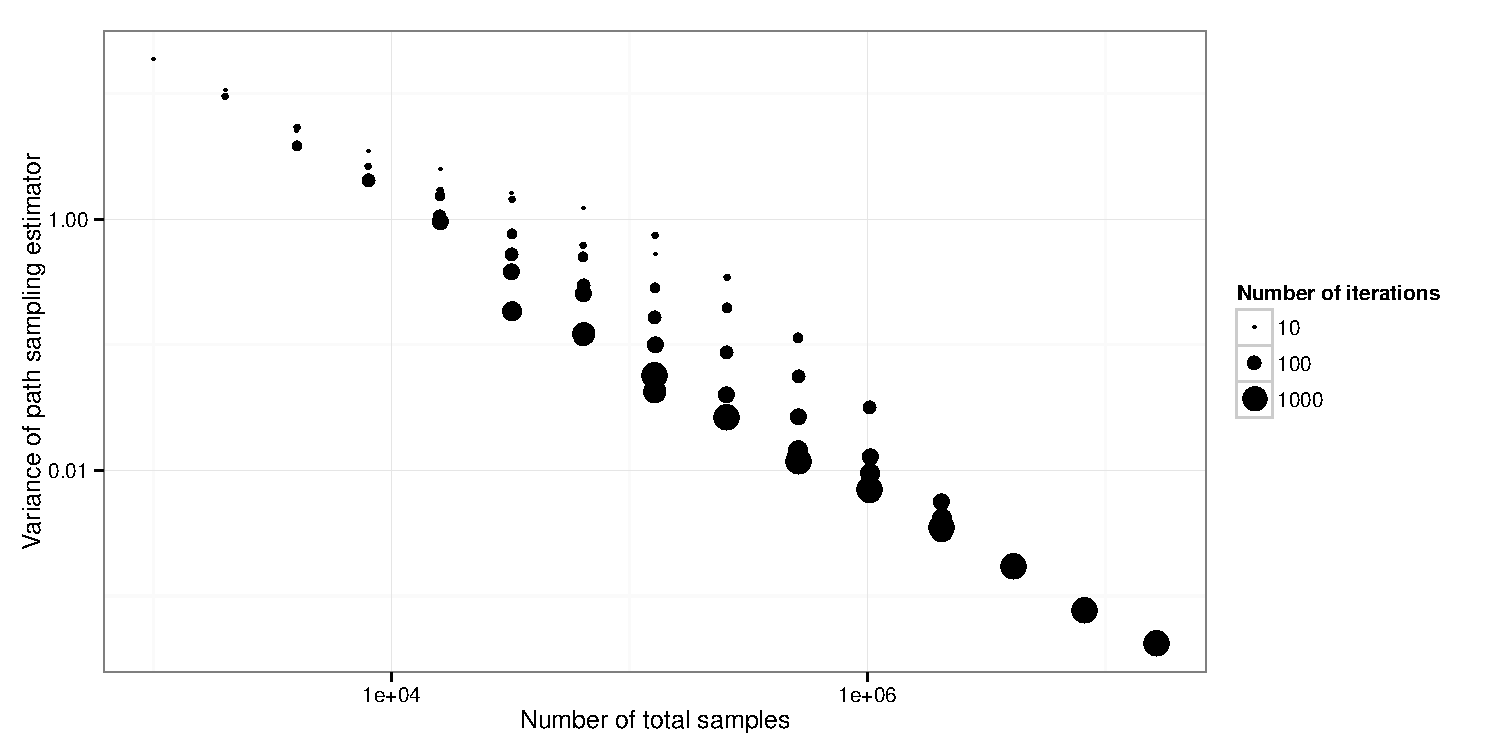
\includegraphics[width=\linewidth]{fig/Particle_Iter_Var}
  \caption{Variance of path sampling estimates and total number of samples
    using the \smc[2] algorithm.}
  \label{fig:particle iter num}
\end{figure}

It can be seen through the nonlinear \ode and the \pet examples that, there is
a trade-off between the number of particles and distributions. Increasing
either of them can improve the accuracy of estimates. We consider a range of
number of particles (from 100 to more than 10,000) and a range of number of
distributions using the prior schedule ($\alpha(t/T) = (t/T)^5$; from as small
as 10 to more than 1,000.) When applied to the simulated data set, the
variance of the path sampling estimates is plotted against the total number of
samples (the product of these two quantities) in figure~\ref{fig:particle iter
  num}. It can be seen that, for the same total number of samples, samplers
with larger number of distributions outperform those with larger number of
particles by a considerable large margin. However, as the number of samples
increase, the difference becomes smaller and smaller. This suggests that it
will be better to first allocate a fixed number of particles, according to
considerations such as computation hardwares. And then use the number of
distributions as a performance parameter to tune the sampler for desired
accuracy. When using the adaptive algorithms proposed in this work, it is
equivalent to tune the value of $\cess^\star$. As shown in
section~\ref{sub:Adaptive specification of distributions}, the relation
between $\cess^\star$ and the variance of estimators provides a predictive way
to configure the samplers.

\paragraph{Fast mixing \mcmc kernels and number of distributions}

As mentioned in section~\ref{sub:Optimal and suboptimal backward kernels}, the
suboptimal backward kernel and its associated incremental weights used in the
above examples could perform poorly if the adjacent distributions are not
close, even when the transition kernel mixes well. However, both fast mixing
kernels and more intermediate distributions (and thus a smoother sequence),
can improve the performance of the sampler. To improve the mixing speed of the
kernel, one can apply multiple passes of \mcmc moves at each iteration. Here
we compare two samplers use the simulated data set, both with 1,000 particles.
One sampler use 10 \mcmc moves at each iteration. The other only use one \mcmc
move but use ten times the number of distributions. The annealing scheme, for
simplicity, is chosen to be $\alpha(t/T) = (t/T)^5$. The results of the path
sampling variance is shown in figure~\ref{fig:fast mcmc iter}. It can be seen
that, given the same total number of samples simulated, using more
distributions almost always outperforms using more \mcmc moves. However, with
sufficient large number of samples, the difference is minimal.

\begin{figure}[t]
  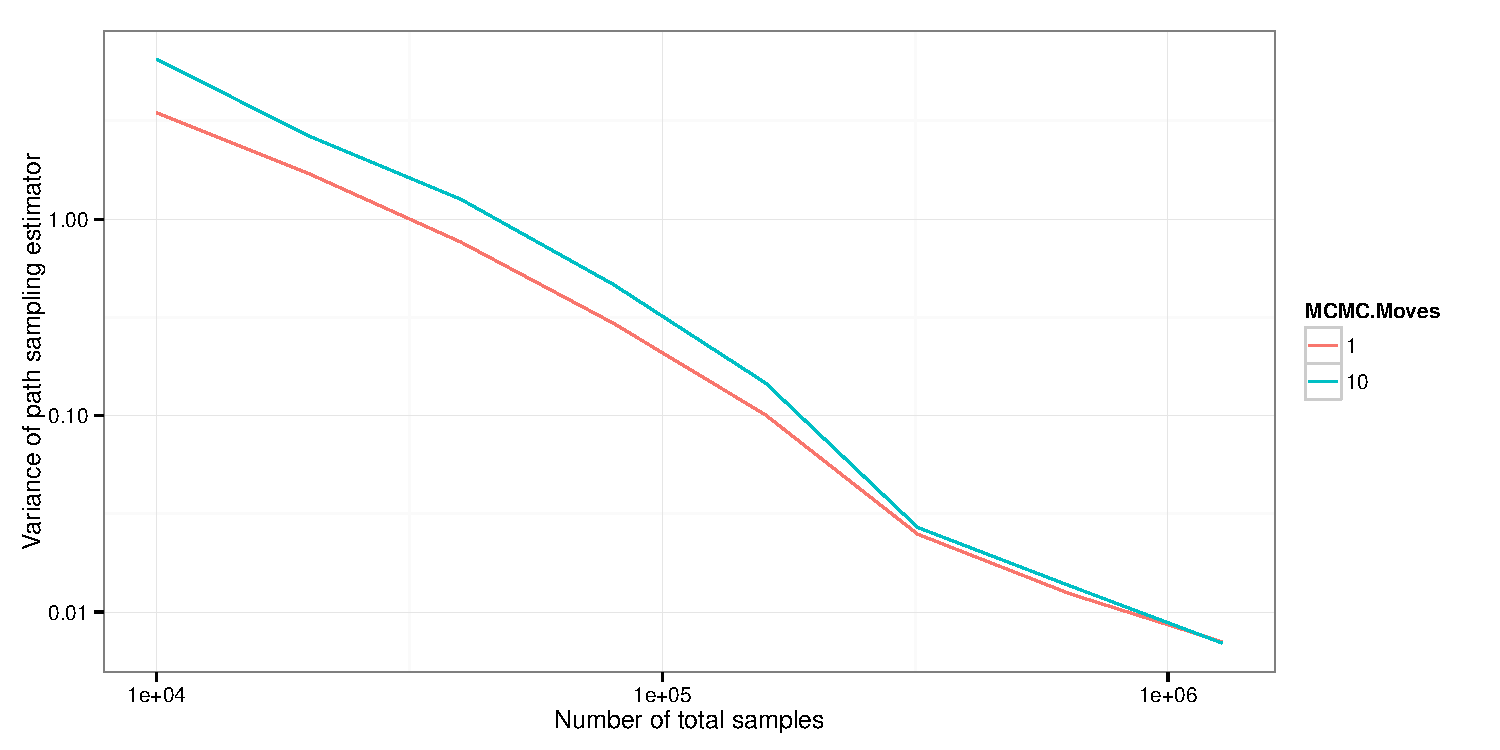
\includegraphics[width=\linewidth]{fig/MCMC_Iter_Var}
  \caption{Variance of path sampling estimates and total number of samples
    using the \smc[2] algorithm. Both samplers use 1,000 particles but with
    different number of distributions and passes of \mcmc moves at each
    iteration}
  \label{fig:fast mcmc iter}
\end{figure}

\paragraph{Real data results}

Finally, the methodology of \smc[2]-\ps was applied to measured positron
emission tomography data using the same compartmental setup as in the
simulations. The data shown in Figure~\ref{fig:petplot} comes from a study
into opioid receptor density in Epilepsy, with the data being described in
detail in \cite{Jiang:2009kf}. It is expected that there will be considerable
spatial smoothness to the estimates of the volume of distribution, as this is
in line with the biology of the system being somewhat regional. Some regions
will have much higher receptor density while others will be much lower,
yielding higher and lower values of the volume of distribution, respectively.
While we did not impose any spatial smoothness but rather estimated the
parameters independently for each time series at each spatial location, as can
be seen, smooth spatial estimates of the volume of distribution consistent
with neurological understanding were found using the approach. This method is
computationally feasible for the entire brain on a voxel-by-voxel basis, due
to the ease of parallelization of the \smc algorithm. In the analysis
performed here 1,000 particles were used, along with an adaptive schedule
using a constant $\cess^\star/N = 0.999$, resulting in about 180 to 200
intermediate distributions. The model selection results are very close to
those obtained by a  previous study of the same data \cite{Zhou2013}, although
the present approach requires much less implementation effort and has roughly
the same computational cost.

\subsection{Summary}

These three illustrative applications have essentially shown three aspects of
using \smc as a generic tool for Bayesian model selection. Firstly, as seen in
the Gaussian mixture model example, all the different variants of \smc
proposed, including both direct and path sampling versions, produce results
which are competitive with other model selection methods such as \rjmcmc and
\pmcmc. In addition, in this somewhat simple example, \smc[2] performs well,
and leads to low variance estimates with no appreciable bias. The effect of
adaptation was studied more carefully in the nonlinear \ode example, and it
was shown that using both adaptive selection of distributions as well as
adaptive proposal variances leads to very competitive algorithms, even against
those with significant manual tuning. This suggests that an automatic process
of model selection using \smc[2] is possible. In the final example,
considering the easy parallelization of algorithms such as \smc[2] suggests
that great gains in variance estimation can be made using settings such as
\gpu computing for application where computational resources are of particular
importance (such as in image analysis as in the PET example). It is also clear
that the negligible cost of the bias reduction techniques described means that
one should always consider using these to reduce the bias inherent in path
sampling estimation.

\section{Discussion}
\label{sec:Bayesian SMC discussion}

It has been shown that \smc is an effective Monte Carlo method for Bayesian
inference for the purpose of model comparison. Three approaches have been
outlined and investigated in several illustrative applications including the
challenging scenarios of nonlinear \ode models and \pet compartmental systems.
The proposed strategy is always competitive and often substantially
outperforms the state of the art in this area.

It has been demonstrated that it is possible to use the \smc algorithms to
estimate the model probabilities directly (\smc[1]), or through individual
model evidence (\smc[2]), or pair-wise relative evidence (\smc[3]). In
addition, both \smc[2] and \smc[3] algorithms can be coupled with the path
sampling estimator.

Among the three approaches, \smc[1] is applicable to very general settings. It
can provide a robust alternative to \rjmcmc when inference on a countable
collection of models is required (and could be readily combined with the
approach of \cite{Jasra:2008bb} at the expense of a little additional
implementation effort). However, like all Monte Carlo methods involving
between model moves, it can be difficult to design efficient algorithms in
practice. The \smc[3] algorithm is conceptually appealing. However, the
existence of a suitable sequence of distributions between two posterior
distributions may not be obvious.

The \smc[2] algorithm, which only involves within-model simulation, is most
straightforward to implement in many interesting problems. It has been shown
to be exceedingly robust in many settings. As it depends largely upon a
collection of within-model \mcmc moves, any existing \mcmc algorithms can be
reused in the \smc[2] framework. However, much less tuning is required because
the algorithm is fundamentally less sensitive to the mixing of the Markov
kernel and it is possible to implement effective adaptive strategies at little
computational cost. With adaptive placement of the intermediate distributions
and specification of the \mcmc kernel proposals, it provides a robust and
essentially automatic model comparison method.

Compared to the \pmcmc algorithm, \smc[2] has greater flexibility in the
specification of distributions. Unlike \pmcmc, where the number and placement
of distributions can affect the mixing speed and hence performance
considerably, increasing the number of distributions will always benefit a
\smc sampler given the same number of particles. When coupled with a path
sampling estimator, this leads to less bias and variance. Compared to its
no-resampling variant, it has been shown that \smc samplers with resampling
can reduce the variance of normalizing constant estimates considerably.

Even after three decades of intensive development, no Monte Carlo method can
solve the Bayesian model comparison problem completely automatically without
any manual tuning. However, \smc algorithms and the adaptive strategies
demonstrated in this paper show that even for realistic, interesting problems,
these samplers can provide good results with very minimal tuning and few
design difficulties. For many applications, they could already be used as near
automatic, robust solutions. For more challenge problems, the robustness of
the algorithms can serve as solid foundation for specific algorithm designs.
